% AUTO-GENERATED by Github-Branch/tools/build_unified_source.ps1.
% Do not edit this file directly: update the transformation manifest instead.
\chapter{Calibration, Model Comparison and Gold-Price Simulation}
\chapterstatus{Edited reuse from Team 8 plus the accepted current diagnostics.
The fitted object is a GLD option surface under the risk-neutral measure
$\mathbb Q$; it is not a direct fit to physical gold spot under $\mathbb P$.
Calibration, data-freeze and out-of-sample claims retain their separate gates.}
\sourceassetnote
\section{LSE Market Inputs and Shared Calibration Architecture}

The introduction defined the modelling objective; this chapter builds the empirical object to which the models will be fitted. It starts from the option chain, constructs implied volatilities, chooses a structured calibration sample, and ends with the market surface that becomes the input for the constrained optimization problem. The target is option-implied information for GLD under $\mathbb Q$. Calling it forward-looking means that current option prices encode market pricing across future maturities; it does not mean that the fitted distribution is an unbiased forecast of realised gold returns under $\mathbb P$. Any use in the corporate valuation is therefore a disclosed conditional scenario interface, not a silent change of measure.
\subsection{From Option Chain to Calibration Dataset}

After the introduction has fixed the role of the present article inside the broader Barrick project, the first concrete object is the market surface. London Strategic Edge (LSE) is the sole market-data source used by the reproducible pipeline \sourcecitation{LondonStrategicEdge2026}. The source-study snapshot records \(S_0=404.77\) for GLD at 20:15:07 UTC on 12 August 2026. It returns 2,477 call records; 445 pass the freshness, maturity, moneyness, and numerical filters, and 64 enter the structured Chebyshev sample across eight expiries. The methodology and historical diagnostics below preserve that snapshot; the current 27 August recalibration used by the unified valuation is reported in the dedicated current-surface subsection.

An important timing issue must be handled explicitly. An option's LSE \texttt{last\_price} can come from a trade older than the current underlying snapshot and may therefore be inconsistent with the current spot. The workflow keeps that field only in the local audit. It treats LSE implied volatility as the observed surface and reconstructs a coherent call price and vega with the Black--Scholes implementation, one snapshot spot, one maturity clock, \(q=0\), and the maturity-specific LSE Treasury rate. Only contracts updated within seven days are eligible. Raw and row-level LSE data remain in a Git-ignored local directory under the provider's redistribution terms; the public repository contains the code, a hashed aggregate manifest, calibrated parameters, aggregate errors, and research figures.

The practical cleaning pipeline performs four tasks:

\begin{enumerate}[leftmargin=8mm, itemsep=2pt]
    \item retain current GLD calls updated no more than seven days before the snapshot;
    \item express every expiry against one snapshot clock and require at least 60 days to maturity;
    \item retain strikes within \(\pm20\%\) of spot and valid positive LSE implied volatilities;
    \item map LSE IV into a no-arbitrage call price and vega, then select the 64-point Chebyshev sample.
\end{enumerate}

The Black--Scholes formula is used here as a consistency map, not as the final explanatory model. This is the same modelling limitation already visible in previous work on gold-price scenarios: a Black--Scholes volatility provides a useful benchmark for a first Monte Carlo exercise, but one constant volatility cannot reproduce the full smile \sourcecitation{BarrickArticle4}. Given the LSE implied volatility \(\sigma_i^{LSE}\), the normalized calibration price is
\begin{equation}
    C_i^{mkt}:=C^{BS}(S_0,K_i,T_i,r_i,q,\sigma_i^{LSE}).
\end{equation}
This construction ensures that the price target and vega share the same timestamp and assumptions. After each richer model is priced, its price is inverted through bisection to obtain the implied-volatility residual shown in the diagnostics.
\subsection{Rate Assignment}

The option-chain response does not carry a risk-free curve in each contract row, but the same LSE API exposes US government-bond yields. The current build requests the 1M, 2M, 3M, 6M, 1Y, 2Y, 3Y, 5Y, 7Y, 10Y, 20Y and 30Y nominal Treasury series. Eleven observations share 24 July 2026; only the 10Y tenor is unavailable on that common date. If \(y(\tau)\) is the reported par yield in decimal form, the documented continuous-rate proxy is
\[
    R(\tau)=\log\!\left(1+y(\tau)\right),
\]
The branch fits a constrained six-parameter Nelson--Siegel--Svensson curve
\[
R_{NSS}(\tau)=\beta_0+\beta_1L_1(\tau/\tau_1)
+\beta_2L_2(\tau/\tau_1)+\beta_3L_2(\tau/\tau_2),
\]
where \(L_1(x)=(1-e^{-x})/x\) and \(L_2(x)=L_1(x)-e^{-x}\). The current
parameter vector, ordered as \(\beta_0,\beta_1,\beta_2,\beta_3,\tau_1,\tau_2\),
is
\[
(0.01739,\;0.01932,\;0.02852,\;0.10328,\;1.41892,\;15.07964).
\]
Its RMSE is 2.37
basis points and its maximum absolute node error is 5.28 basis points. The
fitted zero-rate proxy assigns \(r(T_i)\) to each option maturity; simulations
use quarterly forward rates whose time integrals reproduce the same NSS
discount curve. These are reproducible par-yield-derived proxies, not a
bootstrapped zero-coupon term structure. Crucially, this is a new current LSE
curve owned by the Team~8/unified pipeline; it is not the legacy Team~4 NSS
demonstrator.
\vspace{0.5cm}

\IfFileExists{img/diagnostics/usd_treasury_curve.png}{%
% Asset/code block omitted pending provenance acceptance.

}{}
\vspace{1cm}

Once rates are assigned, each option record contains the quantities needed by the pricing functions:
\[
    (S_0,K_i,T_i,r_i,q,C_i^{mkt},\sigma_i^{imp},\vega_i).
\]
The last component, \(\vega_i\), becomes important in the calibration objective. It converts price errors into a first-order approximation of implied-volatility errors.

\vspace{0.5cm}
\subsection{Sampling the Surface}

Full option surfaces are often irregular. Maturities are listed on discrete expiration dates, strikes are not evenly spaced, and market data can be sparse in some regions. Using the entire filtered surface at every calibration step is possible in principle, but it makes Fourier pricing expensive and can make local refinement more sensitive to noisy or redundant contracts. The article therefore compares two sampling strategies:

\begin{itemize}[leftmargin=8mm, itemsep=2pt]
    \item \textbf{uniform sampling}, which selects observations close to a regular grid in \((T,K)\);
    \item \textbf{Chebyshev sampling}, which places more nodes near the boundaries of the domain.
\end{itemize}

The role of Chebyshev sampling is not only graphical. It gives a criterion for choosing a smaller but structured set of calibration points. Instead of picking fewer contracts arbitrarily, the surface is approximated from nodes that cover the domain and put additional attention near the strike-maturity boundaries. This is useful because a smaller dataset makes calibration faster and often numerically cleaner, while the boundary concentration helps reveal interpolation and extrapolation weaknesses that a regular interior grid could hide. In this article, the 64-point Chebyshev sample is therefore the practical compromise between information coverage and calibration stability.

\IfFileExists{img/diagnostics/sampling_comparison.png}{%
% Asset/code block omitted pending provenance acceptance.

}{}
\subsection{Implied-Volatility Surface}

The filtered dataset is visualized as an implied-volatility surface. This is the object the models try to explain. A flat surface would be consistent with the strongest Black--Scholes assumptions. The observed surface is not flat: it varies across strike and maturity, showing the empirical need for richer dynamics.

\IfFileExists{img/diagnostics/volatility_surface_3d.png}{%
% Asset/code block omitted pending provenance acceptance.

}{}

The surface is not interpreted as a deterministic forecast of future gold prices. It is a market-implied object: it summarizes option prices through the Black--Scholes volatility parameter. The calibration problem is therefore to choose model parameters that reproduce this surface as closely as possible under the chosen stochastic dynamics. Once calibrated, those parameters can become inputs for a Monte Carlo gold-price path generator, replacing a single-volatility GBM block with a stochastic-volatility or jump--stochastic-volatility path model. This is the bridge to the next section: fitting the surface is not just a finance problem, but a constrained optimization problem.

% ===============================
\subsection{Empirical GLD Returns and the Normality Hypothesis}

The option surface is a risk-neutral cross-section, whereas the daily GLD series is a historical diagnostic. Both are obtained from LSE, but they answer different questions. Let \(r_t=100[\log S_t-\log S_{t-1}]\). The null hypothesis is that \(r_t\) is normally distributed. The density comparison and Q--Q plot in Figure~\sourceref{fig:return-normality} make tail departures visible, while Shapiro--Wilk, Jarque--Bera, and D'Agostino \(K^2\) provide complementary hypothesis tests.

\IfFileExists{img/diagnostics/gld_return_normality.png}{%
% Asset/code block omitted pending provenance acceptance.

}{}

% Asset/code block omitted pending provenance acceptance.


All three tests reject. With a large, heterogeneous financial sample, rejection is unsurprising and does not identify a preferred option model. The tests are therefore used only to reject Gaussian adequacy and motivate richer dynamics; relative predictive performance is evaluated separately in the rolling test later in this chapter.
\subsection{Shared Constrained-Optimization Framework}

Chapter 2 ended with the object that must be fitted: a cleaned implied-volatility surface built from market option prices. This chapter explains the optimization language used to fit that surface. It introduces the constrained calibration problem, the KKT conditions that characterize feasible local optima, and the SLSQP logic used later in the numerical calibrations. The toy example is intentionally simple: it isolates feasibility and stationarity before the article returns to Heston, Bates, and Bates--Hawkes prices.
\subsection{Calibration as a Constrained Nonlinear Program}

Let \(\theta\in\R^n\) be a vector of model parameters. For the Heston model,
\[
    \theta_H=(v_0,\kappa,\theta_v,\xi,\rho),
\]
where \(v_0\) is the initial variance, \(\kappa\) the mean-reversion speed, \(\theta_v\) the long-run variance, \(\xi\) the volatility of volatility, and \(\rho\) the correlation between the asset and variance shocks. For the Bates model, the vector is enlarged to
\[
    \theta_B=(v_0,\kappa,\theta_v,\xi,\rho,\lambda,\mu_J,\sigma_J),
\]
where \(\lambda\) is jump intensity and \(\mu_J,\sigma_J\) describe the log-jump distribution.

From the perspective of operational research, this is a nonlinear programming problem of the same class discussed in standard optimization references such as Nocedal and Wright and Boyd and Vandenberghe \sourcecitation{NocedalWright2006,BoydVandenberghe2004}. The generic calibration problem is
\begin{equation}
    \min_{\theta\in\R^n} F(\theta)
    \quad\text{subject to}\quad
    h(\theta)=0,\qquad g(\theta)\geq 0,
\end{equation}
where \(F\) is the calibration loss, \(h\) are equality constraints, and \(g\) are inequality constraints. In the present calibration problem, most admissibility requirements are expressed as bounds and penalties. Examples include positive variances, positive mean-reversion parameters, positive jump volatility, non-negative jump intensity, and \(-1<\rho<1\).

% Asset/code block omitted pending provenance acceptance.


The objective used for calibration is a vega-weighted mean squared error:
\begin{equation}
    F(\theta)
    =
    \frac{1}{N}\sum_{i=1}^N
    \left(
    \frac{C_i^{model}(\theta)-C_i^{mkt}}{\max(\vega_i,\varepsilon)}
    \right)^2,
\end{equation}
where \(\varepsilon>0\) protects the denominator when vega is numerically small. This objective is a computational compromise. Directly minimizing implied-volatility errors would require solving a new implied-volatility inversion for every option at every optimizer step. Dividing the price error by Black--Scholes vega uses the first-order relation
\begin{equation}
    \Delta C \approx \vega \, \Delta\sigma.
\end{equation}
Hence
\begin{equation}
    \Delta\sigma \approx \frac{\Delta C}{\vega}.
\end{equation}
This makes the loss closer to an implied-volatility error while keeping the calibration computationally feasible.
\subsection{KKT Conditions}

The KKT conditions describe what a local constrained optimum must satisfy under regularity assumptions. For the problem in \sourceref{eq:generic-nlp}, adopt the convention
\[
    h(\theta)=0,\qquad g(\theta)\geq0,
\]
and define the Lagrangian
\begin{equation}
    \Lag(\theta,\lambda,\mu)
    =
    F(\theta)
    + \lambda^\top h(\theta)
    - \mu^\top g(\theta),
\end{equation}
with inequality multipliers \(\mu\geq0\).

\begin{theorem}[Karush--Kuhn--Tucker conditions]
Let \(\theta^\star\) be a local solution of \sourceref{eq:generic-nlp}, and assume the relevant constraint qualification holds. Then there exist multipliers \(\lambda^\star\) and \(\mu^\star\) such that
\begin{align}
    \nabla_\theta \Lag(\theta^\star,\lambda^\star,\mu^\star) &= 0,
    &&\text{stationarity}, \\
    h(\theta^\star) &= 0,
    &&\text{equality feasibility}, \\
    g(\theta^\star) &\geq 0,
    &&\text{inequality feasibility}, \\
    \mu^\star &\geq 0,
    &&\text{dual feasibility}, \\
    \mu_j^\star g_j(\theta^\star) &= 0\quad\forall j,
    &&\text{complementary slackness}. 
\end{align}
\end{theorem}

Stationarity says that, at the solution, the gradient of the objective can be balanced by the gradients of the active constraints. Complementary slackness says that an inequality constraint either binds, in which case its multiplier may be positive, or it is slack, in which case its multiplier must be zero.

In model calibration, this matters because many bad parameter proposals are not merely numerically unattractive; they are infeasible. A negative variance, a correlation outside \([-1,1]\), or a negative jump intensity has no acceptable interpretation in the model. SLSQP uses local quadratic approximations while respecting these restrictions.
\subsection{From SQP to SLSQP}

Sequential Quadratic Programming (SQP) solves \sourceref{eq:generic-nlp} by repeatedly replacing the original nonlinear problem with a quadratic approximation. At iteration \(k\), with current parameter vector \(\theta_k\), write a local step \(d\). The objective is approximated by
\begin{equation}
    F(\theta_k+d)
    \approx
    F(\theta_k)
    + \nabla F(\theta_k)^\top d
    + \frac{1}{2} d^\top B_k d,
\end{equation}
where \(B_k\) approximates the Hessian of the Lagrangian. The constraints are linearized:
\begin{align}
    h(\theta_k+d)
    &\approx h(\theta_k)+J_h(\theta_k)d,\\
    g(\theta_k+d)
    &\approx g(\theta_k)+J_g(\theta_k)d.
\end{align}
The local quadratic subproblem is therefore
\begin{align}
    \min_d \quad &
    \nabla F(\theta_k)^\top d
    + \frac{1}{2}d^\top B_kd
    \\
    \text{subject to}\quad &
    h(\theta_k)+J_h(\theta_k)d=0, \nonumber\\
    &
    g(\theta_k)+J_g(\theta_k)d\geq0. \nonumber
\end{align}

SLSQP belongs to this SQP family. In the terminology used here, SQP means Sequential Quadratic Programming; SLSQP is the least-squares variant associated with Kraft's algorithm \sourcecitation{Kraft1988}. The method solves constrained quadratic subproblems using least-squares ideas and then performs a line-search step to decide how far to move:
\begin{equation}
    \theta_{k+1} = \theta_k+\alpha_k d_k,\qquad 0<\alpha_k\leq1.
\end{equation}
The Hessian approximation is updated iteratively, usually through a quasi-Newton update. For the present article, the important point is not the software interface but the logic: the method searches for a better fit while keeping the parameter vector inside an admissible region.

\vspace{0.5cm}


\begin{tcolorbox}[title={Simplified SLSQP loop}, colback=white, boxrule=0.4pt]
\begin{enumerate}[leftmargin=8mm, itemsep=2pt]
    \item Start from a feasible or nearly feasible parameter vector \(\theta_0\).
    \item Evaluate the calibration objective and local derivatives or finite-difference approximations.
    \item Build a quadratic approximation of the objective and linear approximations of the constraints.
    \item Solve the quadratic subproblem for a search direction \(d_k\).
    \item Use a line search to choose \(\alpha_k\), then update \(\theta_{k+1}=\theta_k+\alpha_k d_k\).
    \item Stop when the step, objective improvement, and constraint violation are below tolerance.
\end{enumerate}
\end{tcolorbox}
\vspace{0.5cm}
\subsection{Toy Example}

Consider the problem
\begin{equation}
    \min_{x,y}\; f(x,y)=(x-1)^2+(y-2)^2
    \quad\text{subject to}\quad
    x+y=2,\quad x\geq0,\quad y\geq0.
\end{equation}
The unconstrained minimizer is \((1,2)\), but it violates \(x+y=2\). The constrained solution is the projection of \((1,2)\) onto the line \(x+y=2\), which is
\begin{equation}
    (x^\star,y^\star)=\left(\frac{1}{2},\frac{3}{2}\right).
\end{equation}
Both inequalities are slack, since \(x^\star>0\) and \(y^\star>0\). Therefore their multipliers are zero. For the equality constraint \(h(x,y)=x+y-2=0\), define
\[
    \Lag(x,y,\eta,\mu_1,\mu_2)
    =
    (x-1)^2+(y-2)^2
    +\eta(x+y-2)-\mu_1x-\mu_2y.
\]
At \((1/2,3/2)\),
\[
    \nabla f(x^\star,y^\star)=(-1,-1).
\]
Stationarity becomes
\[
    (-1,-1)+\eta(1,1)-(0,0)=0,
\]
so \(\eta=1\). The KKT conditions are satisfied:
\[
    x^\star+y^\star-2=0,\qquad x^\star>0,\qquad y^\star>0,\qquad
    \mu_1=\mu_2=0.
\]

Now interpret the first SLSQP step. Suppose the algorithm starts from \((x_0,y_0)=(0.2,0.4)\), which violates the equality constraint because \(x_0+y_0-2=-1.4\). Use \(B_0=2I\), which is the exact Hessian of \(f\). The gradient is
\[
    \nabla f(x_0,y_0)=(-1.6,-3.2).
\]
The equality-linearized quadratic subproblem is
\[
    \min_d\; (-1.6,-3.2)^\top d+d^\top d
    \quad\text{subject to}\quad d_x+d_y=1.4.
\]
Solving the KKT system gives \(d=(0.3,1.1)\). Therefore the full step reaches
\[
    (x_1,y_1)=(0.2,0.4)+(0.3,1.1)=(0.5,1.5),
\]
which is already the constrained optimum.

% Asset/code block omitted pending provenance acceptance.


The toy example is deliberately simple, but it shows the same structural idea used in Heston and Bates calibration. The optimizer is not allowed to chase the raw best fit if doing so violates admissible parameter conditions. The local step must balance objective improvement and feasibility.

% ===============================

Chapters 3--5 built the ingredients of the calibration problem: constrained optimization, affine pricing models, and the Hawkes self-exciting jump state. This chapter puts those ingredients into a workflow. It explains how the objective is weighted, how global and local search are combined, and which constraints define the admissible Heston, Bates, and Bates--Hawkes parameter regions.
\subsection{Why Raw Price Errors Are Not Enough}

The pricing models are now defined; calibration decides how they are fitted to the surface. This is where the operational-research discussion becomes practical. The objective function, the parameter bounds, and the initialization strategy determine whether the final result is a meaningful model or only a numerical fit.

Option prices have very different scales. Deep in-the-money contracts can have large dollar prices, while out-of-the-money contracts can be cheap but highly informative about tail risk. If calibration minimizes raw squared price errors,
\[
    \sum_i \left(C_i^{model}(\theta)-C_i^{mkt}\right)^2,
\]
then expensive options tend to dominate the fit. The optimizer may improve the dollar error on high-price contracts while ignoring regions of the volatility smile that are crucial for model interpretation.

The project therefore uses the vega-weighted objective in \sourceref{eq:vega-weighted-objective}. This is a practical operational-research choice: it changes the geometry of the objective so that the optimizer behaves more like it is fitting implied volatilities, but without forcing an implied-volatility inversion inside every objective evaluation.
\subsection{Global Initialization and Local Refinement}

Heston and Bates objectives are not simple convex functions. They contain numerical integration, nonlinear parameter interactions, and regions where different parameter combinations produce similar option prices. A purely local method can converge to a poor local minimum if it starts from an unlucky point.

For this reason, the calibration uses a two-stage design:

\begin{enumerate}[leftmargin=8mm, itemsep=2pt]
    \item \textbf{Differential Evolution.} A global population-based search explores the bounded parameter space and returns a robust candidate.
    \item \textbf{SLSQP.} The global candidate becomes the starting point for local constrained refinement.
\end{enumerate}

This is a pragmatic compromise. Differential Evolution is expensive but more exploratory. SLSQP is faster near a good candidate and can exploit local smoothness. The global stage protects the local optimizer from starting too far away, while SLSQP improves the final local fit under the parameter restrictions described earlier.

The shared machinery is now fixed. The remaining question is incremental: which empirical defect remains after each calibrated model, and which new state variable is needed to address it? The next four chapters answer that question in model order.

% ===============================
\section{Black--Scholes Baseline: Calibration, Errors, and Rejection}

Black--Scholes is the transparent starting point inherited from the foundational article in this research track \sourcecitation{BarrickArticle1}. It supplies the price/IV conversion and vega weights used everywhere else, so its limitations must be measured before a richer model is introduced.

The previous section explained why SLSQP matters: the models are useful only if their parameters can be estimated under economically meaningful restrictions. We now connect that optimization language to the three model families used in the article. The goal is not to document a technical workflow, but to make clear what each model contributes to the gold-price block.
\subsection{Black--Scholes as the Baseline}

The Black--Scholes European call price is
\begin{equation}
    C^{BS}(S,K,T,r,q,\sigma)
    =
    S e^{-qT}N(d_1)-K e^{-rT}N(d_2),
\end{equation}
where
\begin{align}
    d_1 &=
    \frac{\log(S/K)+(r-q+\frac{1}{2}\sigma^2)T}{\sigma\sqrt{T}},\\
    d_2 &= d_1-\sigma\sqrt{T}.
\end{align}
The corresponding vega is
\begin{equation}
    \vega^{BS}
    =
    S e^{-qT} N'(d_1)\sqrt{T}.
\end{equation}

In this article, Black--Scholes has three roles. First, it gives a transparent reference price. Second, it converts option prices into implied volatilities, allowing the surface in Chapter 2 to be drawn and interpreted. Third, it provides the vega term used in the calibration loss \sourceref{eq:vega-weighted-objective}. Its weakness is exactly the reason the article continues: a single volatility parameter cannot reproduce the full strike-maturity geometry of the observed surface.
\subsection{Calibration Choice and Error Tests}

The baseline estimates one constant volatility by minimizing the same vega-weighted loss used for the richer models. The deterministic fit gives \(\widehat\sigma=0.243713\). Price MAE and RMSE are \(0.6375\) and \(0.8156\); IV MAE and RMSE are \(87.78\) and \(117.93\) basis points. Applying normality tests to the 64 market-minus-model IV residuals rejects normality with Shapiro \(p=6.10\cdot10^{-5}\), Jarque--Bera \(p=8.32\cdot10^{-6}\), and D'Agostino \(p=8.24\cdot10^{-5}\). The rejection is secondary to the geometry: a constant volatility leaves a structured smile error.
\subsection{Residual Heatmaps}

After calibration, the model price for each option is converted back into an implied volatility and compared with market implied volatility. The residual is reported as
\begin{equation}
    \text{Residual}_i
    =
    \sigma_i^{mkt}-\sigma_i^{model}.
\end{equation}
Plotting residuals over maturity and moneyness helps identify systematic model failures. A good calibration should not only minimize a scalar loss; it should also avoid structured residual patterns that reveal missing model mechanisms.

The residual figures are placed directly beside the relevant calibrations: Heston in Figure~\sourceref{fig:heston-residuals}, Bates in Figure~\sourceref{fig:bates-residuals}, and full Bates--Hawkes in Figure~\sourceref{fig:bates-hawkes-residuals}. Read together with Tables~\sourceref{tab:model-parameters}--\sourceref{tab:model-errors}, they show both the improved residual scale of the refreshed full model and the additional discontinuous tail-risk mechanism used for scenario design.

\IfFileExists{img/diagnostics/black_scholes_residual_heatmap.png}{%
% Asset/code block omitted pending provenance acceptance.

}{}

\IfFileExists{img/diagnostics/black_scholes_volatility_smile.png}{%
% Asset/code block omitted pending provenance acceptance.

}{}
\subsection{Why Constant Volatility Is Not Sufficient}

Black--Scholes remains essential as a numerical coordinate system, but the residual map and smile slices show that one \(\sigma\) cannot absorb maturity- and strike-dependent variance expectations. The following section therefore introduces a latent mean-reverting variance state rather than trying to repair the same constant-volatility law with a different optimizer.

% ===============================
\section{Heston: Stochastic Variance, Calibration, and Residual Structure}

The preceding chapter isolated the failure of constant volatility. Heston is the smallest affine upgrade that changes the variance law itself: it embeds the CIR-style mean-reverting state motivated by the earlier gold-volatility study \sourcecitation{BarrickArticle6}.
\subsection{Heston: Adding Stochastic Variance}

Heston replaces constant volatility with a stochastic variance process:
\begin{align}
    \frac{\dd S_t}{S_t} &= (r-q)\dd t+\sqrt{v_t}\dd W_t^S,\\
    \dd v_t &= \kappa(\theta_v-v_t)\dd t+\xi\sqrt{v_t}\dd W_t^v,\\
    \dd\langle W^S,W^v\rangle_t &= \rho\dd t.
\end{align}
The variance follows a square-root diffusion. Mean reversion is controlled by \(\kappa\), the long-run variance by \(\theta_v\), volatility of volatility by \(\xi\), and return-volatility asymmetry by \(\rho\).

For option calibration, it is more efficient to price through the characteristic function of \(\log S_T\) than to simulate a large number of paths at every parameter update. In affine form, the characteristic function can be written as
\begin{equation}
    \varphi_H(u;T)
    =
    \exp\left(
        \ii u\log S_0 + C(u,T)\theta_v + D(u,T)v_0 + \ii u(r-q)T
    \right),
\end{equation}
where \(C\) and \(D\) are Riccati-type functions. A single-integral pricing formula then gives
\begin{equation}
    C^{Heston}
    =
    \frac{S_0e^{-qT}-Ke^{-rT}}{2}
    +
    \frac{1}{\pi}\int_0^\infty
    \operatorname{Re}
    \left[
        \frac{e^{-rT}\left(\varphi_H(u-\ii)-K\varphi_H(u)\right)}
        {\ii u K^{\ii u}}
    \right]\dd u.
\end{equation}
This is the first major upgrade over Black--Scholes: volatility is no longer fixed. It becomes a state variable, and the model can generate a curved implied-volatility surface rather than a flat one.
\subsection{Heston Calibration}

The Heston calibration vector is
\[
    \theta_H=(v_0,\kappa,\theta_v,\xi,\rho).
\]
The working bounds are approximately:
\begin{align}
    v_0 &\in [10^{-4},1],&
    \kappa &\in [0.1,10],&
    \theta_v &\in [10^{-4},1],\\
    \xi &\in [0.01,15],&
    \rho &\in [-0.99,0.99].
\end{align}
These are not claims that the true parameters must lie exactly in those intervals. They are numerical guardrails. Without such bounds, local optimizers may test unstable or meaningless parameter values while trying to reduce the objective.

The calibration code also imposes the Feller condition
\begin{equation}
    2\kappa\theta_v-\xi^2\geq0,
\end{equation}
which ensures that the CIR variance process stays strictly positive under the classical boundary classification. This is deliberately stricter than many unconstrained implied-volatility calibrations. In the code, parameter proposals with \(2\kappa\theta_v-\xi^2<0\) receive a large objective penalty, so the reported Heston, Bates, and Bates--Hawkes calibrations must satisfy the same variance-admissibility rule. The residual heatmaps and smile plots are diagnostic evidence collected in the later comparison sections and in the current LSE insert to this chapter.

The 12 August LSE fit is \(v_0=0.06666\), \(\kappa=2.05558\), \(\theta_v=0.04805\), \(\xi=0.18453\), and \(\rho=0.06951\). The Feller gap is \(0.16350>0\). Price RMSE falls to \(0.6317\), and IV RMSE falls to \(94.44\) bp. Residual normality is still rejected (Shapiro \(p=0.0128\), Jarque--Bera \(p=0.0146\), D'Agostino \(p=0.0112\)), so the additional variance state improves scale without eliminating systematic distributional misspecification.

\IfFileExists{img/diagnostics/heston_residual_heatmap.png}{%
% Asset/code block omitted pending provenance acceptance.

}{}

\IfFileExists{img/diagnostics/heston_volatility_smile.png}{%
% Asset/code block omitted pending provenance acceptance.

}{}
\subsection{Why Stochastic Variance Is Still Not Sufficient}

Heston reduces the smooth smile error and creates endogenous volatility dynamics, but its paths remain continuous. The remaining short-maturity and tail residuals can be represented only indirectly through the diffusion parameters. The next model adds an explicit discontinuous return channel and then checks whether that mechanism earns its extra parameters.

% ===============================
\section{Bates: Independent Jumps, Calibration, and Tail Errors}

Heston explains changing variance but not discontinuous repricing. Bates adds a compensated compound-Poisson block to the same affine diffusion, following the jump and Fourier foundations developed in the preceding theoretical article \sourcecitation{BarrickArticle7}.

\vspace{0.5cm}
\subsection{Bates: Adding Jump Risk}

The Bates model augments Heston with a lognormal jump component. Under the risk-neutral measure,
\begin{align}
    \frac{\dd S_t}{S_{t^-}}
    &=
    (r-q-\lambda k)\dd t+\sqrt{v_t}\dd W_t^S+(e^J-1)\dd N_t,\\
    \dd v_t
    &=
    \kappa(\theta_v-v_t)\dd t+\xi\sqrt{v_t}\dd W_t^v,
\end{align}
where \(N_t\) is a Poisson process with intensity \(\lambda\), \(J\sim\mathcal{N}(\mu_J,\sigma_J^2)\), and
\begin{equation}
    k = \E^\Q[e^J-1]
      = \exp\left(\mu_J+\frac{1}{2}\sigma_J^2\right)-1.
\end{equation}
The compensator \(-\lambda k\) prevents the jump term from creating an arbitrage drift under the risk-neutral pricing measure.

Because the jump component is independent of the Heston diffusion component in the Bates specification used here, the characteristic function factors:
\begin{equation}
    \varphi_B(u;T)
    =
    \varphi_H(u;T)
    \exp\left[
        \left(
        \ii u\omega
        +
        \lambda
        \left(
            e^{\ii u\mu_J-\frac{1}{2}u^2\sigma_J^2}-1
        \right)
        \right)T
    \right],
\end{equation}
with
\[
    \omega=-\lambda\left(\exp\left(\mu_J+\frac{1}{2}\sigma_J^2\right)-1\right).
\]
The same Fourier-pricing logic used for Heston can then be reused by replacing \(\varphi_H\) with \(\varphi_B\). Economically, the additional jump terms give the model a direct way to represent discontinuous movements and tail-sensitive option prices.

\paragraph{How the jump layer reallocates fitted variability.}
Adding jumps does not literally create a second diffusion-volatility process. It separates return variation into a continuous stochastic-variance channel and a discontinuous jump channel. For log price \(X_t=\log S_t\), the quadratic variation has the schematic decomposition
\begin{equation}
    [X]_t
    =
    \int_0^t v_s\,\dd s
    +
    \sum_{0<s\leq t}(\Delta X_s)^2.
\end{equation}
The first term is generated by the Heston diffusion and the second by jump arrivals and jump sizes. Once the second channel is available, the optimizer no longer needs the Heston block to reproduce every short-maturity tail and skew feature. The diffusion parameters can therefore fall because part of the option-implied variation is reallocated to \((\lambda,\mu_J,\sigma_J)\). This is a joint-identification effect, not evidence that the underlying economic variance mechanically falls whenever jumps are added.

\subsection{Bates Calibration}

Bates extends Heston by adding three jump parameters:
\[
    \theta_B=(v_0,\kappa,\theta_v,\xi,\rho,\lambda,\mu_J,\sigma_J).
\]
The working bounds for the jump layer are:
\[
    \lambda\in[0,5],\qquad
    \mu_J\in[-0.5,0.5],\qquad
    \sigma_J\in[10^{-4},0.5].
\]
The jump component gives the model additional flexibility, especially at short maturities and in skewed regions of the surface. This flexibility is useful but creates identification risk. For example, high volatility of volatility and high jump volatility can both help explain fat tails. The calibration should therefore be read together with residual plots, parameter plausibility, and robustness checks.

The 12 August fit is \(v_0=0.05899\), \(\kappa=4.68004\), \(\theta_v=0.04787\), \(\xi=0.51835\), \(\rho=0.05882\), \(\lambda=1.20287\), \(\mu_J=0.05062\), and \(\sigma_J=0.05987\), with Feller gap \(0.17941\). Price RMSE is \(0.5364\) and IV RMSE is \(78.13\) bp. Residual normality remains rejected (Shapiro \(p=0.0116\), Jarque--Bera \(p=1.28\cdot10^{-4}\), D'Agostino \(p=6.59\cdot10^{-4}\)).

\vspace{1cm}
\subsection{Smile Slices}

Residual heatmaps give a global view, but smile slices make the fit easier to inspect maturity by maturity. Each panel compares market implied volatilities with the model-implied smile for a given expiration.

The Bates smile slices are shown in Figure~\sourceref{fig:bates-smile}, and the full Bates--Hawkes slices are shown in Figure~\sourceref{fig:bates-hawkes-smile}. Smile slices are especially useful for detecting overfitting. A model may reduce average residuals while producing an implausible curve shape in a sparse maturity bucket. The refreshed full-model panels show where the lower aggregate error comes from and where maturity-specific deviations remain.

\IfFileExists{img/diagnostics/bates_residual_heatmap.png}{%
% Asset/code block omitted pending provenance acceptance.

}{}

\IfFileExists{img/diagnostics/bates_volatility_smile.png}{%
% Asset/code block omitted pending provenance acceptance.

}{}
\subsection{Why Independent Jump Arrivals Are Not Sufficient}

Bates improves the fit and assigns part of tail variation to jumps, but its arrival clock is memoryless: a jump does not alter the conditional probability of another jump. The final model asks whether the remaining residual structure is better represented when arrivals cluster through a stationary self-exciting intensity.

% ===============================
\section{Full Bates--Hawkes: Self-Excitation, Calibration, and Model Tests}

The Bates chapter left one specific restriction: jump times are independent. The exponential Hawkes layer replaces the constant arrival rate with a finite-dimensional self-exciting state while retaining Heston variance, affine pricing, and a direct comparison on the same LSE calls.

The preceding sections moved from Black--Scholes to Heston and then to Bates. This progression relaxes one rigid assumption at a time: constant volatility becomes stochastic variance, and continuous diffusion paths receive discontinuous jumps. One structural restriction still remains in the standard Bates layer. Jump times are generated by a homogeneous Poisson process, so the probability of a market shock tomorrow is independent of whether a shock occurred today.

Empirical financial data often display event clustering. Large price moves, liquidity shocks, and order-book imbalances tend to occur in concentrated windows rather than as isolated independent events. After a large downward move, margin calls, stop-loss orders, liquidity withdrawals, volatility-targeting flows, and dealer hedging can temporarily raise the likelihood of further moves. To represent this feedback mechanism, the constant Poisson intensity can be replaced by a stochastic conditional intensity that depends on the past history of the jump process.

This chapter is a modelling chapter, not a calibration chapter. It defines the Hawkes state variable and the available Bates--Hawkes routes. The numerical calibration order remains in Chapter 6: Heston first, Bates second, and Hawkes only after those benchmarks have been fitted and inspected.
\subsection{Limits of Poisson Arrivals}

In the jump-diffusion model of Chapter 4, the jump arrival process \(\{N_t\}_{t\geq0}\) has constant intensity \(\lambda\). For an infinitesimal interval \([t,t+\dd t]\),
\begin{equation}
    \Q(\dd N_t=1\mid\mathcal{F}_t)=\lambda\,\dd t.
\end{equation}
The model is memoryless: once a jump has occurred, the future jump intensity remains unchanged. This is analytically convenient and useful as a first approximation, but it cannot represent clustered market stress.

The Hawkes idea is to promote the intensity itself to a stochastic process \(\lambda_t\). The model then answers a different question: not only how large jumps are, but how the arrival rate of future jumps changes after past events. This is why Hawkes belongs naturally in the present article. Earlier articles developed the general theory of jump processes and stochastic volatility; here the focus is calibration and model design for the Bates jump layer.
\subsection{Mathematical Definition}

A one-dimensional Hawkes process is a simple point process \(\{N_t\}_{t\geq0}\) with stochastic conditional intensity
\begin{equation}
    \lambda_t
    =
    \bar{\lambda}+\int_0^{t^-}\mu(t-s)\,\dd N_s,
\end{equation}
where \(\bar{\lambda}>0\) is the mean-reversion baseline and \(\mu(\tau)\geq0\) is the excitation kernel. The selected option model also allows the initial state \(\lambda_0\) to differ from this baseline. Equivalently, writing the strictly past jump times as \(\tau_i<t\),
\begin{equation}
    \lambda_t
    =
    \bar{\lambda}+\sum_{\tau_i<t}\mu(t-\tau_i)
\end{equation}
in the stationary initialization.

The exponential kernel is the most useful specification for this article:
\begin{equation}
    \mu(\tau)=\alpha e^{-\beta\tau},
    \qquad
    \alpha>0,\quad \beta>0.
\end{equation}
It gives
\begin{equation}
    \lambda_t
    =
    \bar{\lambda}+(\lambda_0-\bar{\lambda})e^{-\beta t}
    +\sum_{\tau_i<t}\alpha e^{-\beta(t-\tau_i)}.
\end{equation}
Each arrival increases the intensity by \(\alpha\); in the absence of further arrivals, the excess intensity decays back toward \(\bar{\lambda}\) at speed \(\beta\).

\IfFileExists{img/diagnostics/hawkes_intensity_comparison.png}{%
% Asset/code block omitted pending provenance acceptance.

}{}
\subsection{Branching Ratio and Stationarity}

The expected number of direct descendants produced by a single event is the branching ratio
\begin{equation}
    n=\int_0^\infty \mu(s)\,\dd s.
\end{equation}
For the exponential kernel,
\begin{equation}
    n=\int_0^\infty \alpha e^{-\beta s}\,\dd s=\frac{\alpha}{\beta}.
\end{equation}
Stationarity requires
\begin{equation}
    \alpha<\beta.
\end{equation}
If \(\alpha\geq\beta\), the model is critical or supercritical in the branching-process sense. The expected cluster size is no longer finite, and the process does not admit the same stationary interpretation. Financially, this should be read as an unstable feedback regime inside the model, not as a deterministic prediction of market collapse.

\paragraph{Compensator and martingale structure.}
The compensator of the process is
\begin{equation}
    \Lambda_t=\int_0^t\lambda_s\,\dd s.
\end{equation}
Then
\begin{equation}
    M_t=N_t-\Lambda_t
    =
    N_t-\int_0^t\lambda_s\,\dd s
\end{equation}
is a local martingale. For \(0\leq s<t\),
\begin{equation}
    \E\!\left[N_t-N_s\mid\mathcal{F}_s\right]
    =
    \E\!\left[\int_s^t\lambda_u\,\dd u\mid\mathcal{F}_s\right].
\end{equation}
This is the self-exciting counterpart of the Poisson identity \(\E[N_t-N_s]=\lambda(t-s)\). The difference is structural: the Poisson compensator is deterministic, while the Hawkes compensator is random and adapted to the information generated by past events.

\paragraph{Markovian intensity dynamics.}
The exponential kernel makes the intensity Markovian. Between arrivals, the intensity decays deterministically; at an arrival time, it jumps upward. In differential form,
\begin{equation}
    \dd\lambda_t
    =
    \beta(\bar{\lambda}-\lambda_t)\,\dd t+\alpha\,\dd N_t.
\end{equation}
The pair \((N_t,\lambda_t)\) is therefore a piecewise-deterministic Markov process, even though \(N_t\) alone is not Markovian. This mirrors the Heston construction: a richer observable process becomes tractable once the state space is enlarged with a latent variance or intensity factor.

\paragraph{Stationary mean intensity.}
Taking expectations in \sourceref{eq:hawkes-intensity-sde} gives
\begin{equation}
    \frac{\dd}{\dd t}\E[\lambda_t]
    =
    \beta\bar{\lambda}-(\beta-\alpha)\E[\lambda_t].
\end{equation}
Under \(\alpha<\beta\),
\begin{equation}
    \E[\lambda_\infty]
    =
    \frac{\beta\bar{\lambda}}{\beta-\alpha}
    =
    \frac{\bar{\lambda}}{1-n}.
\end{equation}
The long-run event rate is the exogenous baseline amplified by the factor \(1/(1-n)\). The closer \(n\) is to one, the more endogenous the jump activity becomes.
\subsection{From Bates to Bates--Hawkes}

The Bates model uses a constant jump intensity \(\lambda\). The Bates--Hawkes extension replaces that constant by the stochastic process \(\lambda_t\):
\begin{align}
    \frac{\dd S_t}{S_{t^-}}
    &=
    (r-q-\lambda_t k)\,\dd t
    +\sqrt{v_t}\,\dd W_t^S
    +(e^J-1)\,\dd N_t,\\
    \dd v_t
    &=
    \kappa(\theta_v-v_t)\,\dd t+\xi\sqrt{v_t}\,\dd W_t^v,\\
    \dd\lambda_t
    &=
    \beta(\bar{\lambda}-\lambda_t)\,\dd t+\alpha\,\dd N_t,
\end{align}
with \(J\sim\mathcal{N}(\mu_J,\sigma_J^2)\), \(k=\E^\Q[e^J-1]\), and \(N_t\) now having conditional intensity \(\lambda_t\). The compensator in the drift becomes local in time: the model subtracts \(\lambda_t k\) rather than \(\lambda k\).

This specification changes the interpretation of the jump layer. In Bates, \(\lambda\) measures the average arrival rate of independent jumps. In Bates--Hawkes, \(\bar{\lambda}\) is the exogenous mean-reversion baseline, \(\lambda_0\) is the intensity observed at the calibration origin, \(\alpha\) is the upward intensity jump after an event, and \(\beta\) controls the decay speed. The branching ratio \(n=\alpha/\beta\) measures endogenous clustering and the stationary mean is \(\bar{\lambda}/(1-n)\) when \(n<1\).

\paragraph{Hawkes calibration routes and comparison rule.}
The code now exposes four distinct calibration routes, collected here because they should not be interpreted as interchangeable estimates. \emph{Exponential point-process likelihood} estimates a baseline, excitation size, and decay rate from observed event times. \emph{Rough power-law likelihood} uses the regularized kernel \(\mu(\tau)=\alpha(\tau+c)^{-(1+\gamma)}\), with \(0<\gamma<1\), to diagnose longer-lived event memory. \emph{Exact constant-volatility option calibration} uses the affine exponential-Hawkes transform but replaces Heston variance by one diffusion volatility; on the current LSE sample it returns \(\sigma=0.22448\) and a branching ratio of approximately \(0.00460\), so it is useful for validation rather than as the final model. Finally, \emph{full affine Heston--Hawkes calibration} combines stochastic variance and the exact exponential-Hawkes jump transform on the same LSE GLD option sample used by Heston and Bates. Only this fourth route enters the cross-model tables and figures. The likelihood fits require event times rather than option prices, while the constant-volatility benchmark has a different diffusion block; comparing either of them directly with Heston and Bates would therefore confound model fit with a change of target or state variables.

This comparison rule also determines the empirical interpretation. The current LSE constrained run estimates a branching ratio of \(0.41375\), above the imposed 0.02 floor and below the instability boundary, and the full affine model improves the in-sample price and implied-volatility errors relative to Bates. This is evidence that the self-exciting layer is useful for this cross-section; it is not, by itself, an out-of-sample or time-series proof of persistent clustering.
\subsection{Exact Affine Pricing of the Self-Exciting Jump Layer}

The stationary-intensity proxy replaces the path-dependent intensity by a constant. The exponential-kernel dynamics \sourceref{eq:hawkes-intensity-sde} are, however, \emph{affine}, and this is exactly the structure that made Heston and Bates tractable through a characteristic function. Pricing the self-exciting layer therefore does not require simulation; it requires solving a small system of ordinary differential equations. In the selected full model, the diffusion factor below is the Heston characteristic function, not a constant-volatility substitute.

Write \(X_t=\ln S_t\). Because the Brownian diffusion and the jump block are driven by independent sources, the characteristic function of \(X_T\) factorizes,
\begin{equation}
    \phi_{X_T}(u)=\E^\Q\!\big[e^{iuX_T}\big]=\phi_{\mathrm{diff}}(u)\,\phi_{\mathrm{jump}}(u),
\end{equation}
where \(\phi_{\mathrm{diff}}\) is the jump-free Black--Scholes or Heston characteristic function of Chapter 4, and \(\phi_{\mathrm{jump}}\) collects the risk-neutral compensated jump contribution \(\sum_{j=1}^{N_T}J_j-k\int_0^T\lambda_s\,\dd s\).

\paragraph{Riccati system.}
Conditioning on the initial intensity \(\lambda_0\), the affine structure yields
\begin{equation}
    \phi_{\mathrm{jump}}(u)=\exp\!\big(A(u,T)+B(u,T)\,\lambda_0\big),
\end{equation}
where \(A\) and \(B\) solve, forward in \(\tau\),
\begin{align}
    \frac{\dd B}{\dd\tau}
    &=
    \psi_J(u)\,e^{\alpha B}-\beta B-iuk-1,
    \\
    \frac{\dd A}{\dd\tau}
    &=
    \beta\bar{\lambda}\,B,
    \qquad A(0)=B(0)=0,
\end{align}
with the log-normal jump transform \(\psi_J(u)=\exp\!\big(iu\mu_J-\tfrac12\sigma_J^2u^2\big)\) and compensator \(k=e^{\mu_J+\sigma_J^2/2}-1\). The nonlinear term \(e^{\alpha B}\) is the signature of self-excitation: setting \(\alpha=0\) linearizes \sourceref{eq:hawkes-riccati-B} and collapses it to the constant-intensity Bates jump transform in closed form. The system is integrated numerically with a vectorized fourth-order Runge--Kutta scheme; only \sourceref{eq:hawkes-riccati-B} is genuinely nonlinear, and \(A\) follows by quadrature. The implementation calibrates \(\lambda_0\) separately from \(\bar{\lambda}\), allowing the initial option-implied intensity to differ from its long-run baseline.

\paragraph{Consistency limits.}
The construction is pinned down by limits that must hold exactly and that therefore double as implementation tests:
\begin{itemize}[leftmargin=8mm, itemsep=2pt]
    \item at \(u=0\) one has \(B\equiv0\) and \(A\equiv0\), so \(\phi_{X_T}(0)=1\);
    \item evaluated at \(u=-i\) the jump transform equals one, which is precisely the martingale condition \(\E^\Q[S_T]=S_0e^{(r-q)T}\);
    \item \(\alpha=0\) with constant \(\lambda_0\) reproduces the Bates price, while \(\lambda_0=0\) removes the jumps and returns Black--Scholes (or Heston).
\end{itemize}
A sign error in the drift, the compensator, or the jump transform would break one of these identities.

\paragraph{From transform to price.}
European options follow from \(\phi_{X_T}\) by Fourier inversion. The accompanying code uses the COS method of Fang and Oosterlee~\sourcecitation{FangOosterlee2008}, which expands the risk-neutral density in a cosine series on a truncation range fixed by the first cumulants and recovers every strike of a maturity from a single evaluation of the characteristic function. Because the Riccati system is solved once per maturity rather than once per option, the exact engine is only modestly more expensive than the Bates benchmark while remaining a genuine path-dependent Hawkes price. This affine route follows the self-exciting jump-diffusion construction of Souto Arias, Cirillo and Oosterlee~\sourcecitation{SoutoArias2023}.

\paragraph{From rough likelihood to rough option pricing.}
The rough likelihood calibration implemented for event diagnostics does not by itself produce rough-Hawkes option prices. The exponential kernel is the Markovian special case that makes \((N_t,\lambda_t)\) finite-dimensional and reduces the jump transform to \sourceref{eq:hawkes-riccati-B}--\sourceref{eq:hawkes-riccati-A}. A power-law kernel instead leads to a Riccati--Volterra problem. A future pricing extension could approximate that kernel by a finite sum of exponentials through Markovian lifting, using the rough-volatility background developed in \sourcecitation{MessinaSoriano2026}; this additional construction is outside the present comparison.

The Hawkes block has therefore defined the self-exciting state variable, the stability restriction, the proxy baseline, the exact affine transform, and the rough-kernel extension. The following subsections return to calibration in benchmark order: Heston first, Bates second, and Hawkes only after the constant-intensity jump model has been established.

% ===============================
\subsection{Bates--Hawkes Calibration}

Hawkes calibration comes after Heston and Bates, not before them. The reason is practical: Heston defines the stochastic-volatility benchmark, Bates adds a constant-intensity jump benchmark, and only then can a self-exciting intensity be judged against a meaningful reference. Starting from Hawkes without those two baselines would make the extra parameters look more informative than they really are.

The full Bates--Hawkes vector expands the Bates parameters from
\[
    \theta_B=(v_0,\kappa,\theta_v,\xi,\rho,\lambda,\mu_J,\sigma_J)
\]
to
\[
    \theta_{BH}
    =
    (v_0,\kappa,\theta_v,\xi,\rho,\lambda_0,\bar{\lambda},n,\beta,\mu_J,\sigma_J),
\]
with \(\alpha=n\beta\), and the admissible region
\[
    \lambda_0>0,\qquad \bar{\lambda}>0,\qquad 0\leq n<1,\qquad \beta>0,\qquad \sigma_J>0.
\]
Optimizing the branching ratio directly and mapping \(\alpha=n\beta\) enforces \(\alpha<\beta\) by construction. This avoids asking SLSQP to repair unstable Hawkes proposals after they have already entered the expensive pricing routine.

\paragraph{Bates--Hawkes calibration routes.}
The code exposes three Bates--Hawkes routes before the final option-model choice is made, and they are not interchangeable. The exact calibration prices options with the affine Hawkes transform, but in the benchmark version it uses one constant volatility instead of the Heston variance state. The exponential-kernel route estimates a Markovian self-exciting intensity,
\[
    \phi(t)=\alpha e^{-\beta t}, \qquad n=\frac{\alpha}{\beta}<1,
\]
so it has a simple stationarity condition and can be embedded in the affine Bates--Hawkes pricer. The rough-kernel route replaces the exponential decay with a slower power-law decay; it is useful for checking whether jump clustering has long memory, but it is less convenient for the finite-dimensional Fourier/COS pricing stack used in this report. Table~\sourceref{tab:hawkes-methods} reports the three calibration routes side by side.
\vspace{0.5cm}
% Asset/code block omitted pending provenance acceptance.

\vspace{0.5cm}
The preferred Bates--Hawkes specification is therefore the full affine Heston--Hawkes model with an exponential kernel. It is the only route that keeps the Heston variance state, enforces the Feller guard, enforces Hawkes stationarity through \(0\leq n<1\), calibrates to the GLD option surface, and still gives a coherent self-exciting jump law for path simulation. In the refreshed deterministic run it also produces the smallest in-sample error among the reported constrained models.

The practical objective remains aligned with the vega-weighted workflow:
\begin{equation}
    F(\theta_{BH})
    =
    \frac{1}{M}\sum_{i=1}^M
    \left(
        \frac{C_i^{BH}(\theta_{BH})-C_i^{mkt}}{\vega_i^{BS}}
    \right)^2,
\end{equation}
where parameter bounds enforce positivity and \(0\leq n<1\). The engine reproduces the Bates and Black--Scholes limits, satisfies \(\phi(0)=1\), the martingale identity, and put--call parity, and agrees with independent Fourier formulations. The constant-volatility implementation additionally agrees with an Ogata-thinning Monte Carlo check and is retained only as a method benchmark.

The selected full model should not be interpreted as a mechanical claim that Hawkes always improves option-surface fit. Its role is narrower: it is the only Hawkes route that is both option-calibrated and structurally comparable with Heston and Bates after Feller and stationarity restrictions are imposed. The later residual analysis therefore checks whether the lower scalar error is accompanied by a credible geometry rather than treating additional parameters as sufficient evidence.
\vspace{0.5cm}
\paragraph{Parameter reallocation after adding jumps.}
The comparison with standalone Heston makes the two-channel interpretation in \sourceref{eq:quadratic-variation-split} visible. Once a jump channel is added, the optimizer can explain part of the short-maturity tail and skew through jump arrivals and jump sizes rather than through the continuous variance process alone. The relevant interpretation is therefore not that volatility mechanically falls when jumps are introduced. It is that the fitted model reallocates variation between a continuous stochastic-variance channel and a discontinuous jump channel, while the Feller guard prevents the variance block from reaching an inadmissible square-root diffusion region. In the current full Bates--Hawkes specification, the estimated branching ratio \(n=0.41375\) couples this reallocation with a stationary self-exciting arrival mechanism.

% Asset/code block omitted pending provenance acceptance.


The selected full fit has \(v_0=0.04786\), \(\kappa=4.66958\), \(\theta_v=0.04356\), \(\xi=0.63755\), \(\rho=-0.12791\), \(\lambda_0=2.14551\), \(\bar\lambda=1.13699\), \(n=0.41375\), \(\alpha=3.57088\), \(\beta=8.63045\), \(\mu_J=0.05608\), and \(\sigma_J=0.06440\). The Feller gap \(0.000351\) and \(n<1\) satisfy the imposed admissibility rules. Price RMSE is \(0.4076\), and IV RMSE is \(61.02\) bp. All three residual-normality tests still reject; in particular, Jarque--Bera \(p=1.51\cdot10^{-11}\). The scalar improvement is therefore real in sample, but the remaining heavy-tailed residual law prevents an overstatement of adequacy.

\IfFileExists{img/diagnostics/bates_hawkes_residual_heatmap.png}{%
% Asset/code block omitted pending provenance acceptance.

}{}

\IfFileExists{img/diagnostics/bates_hawkes_volatility_smile.png}{%
% Asset/code block omitted pending provenance acceptance.

}{}
\subsection{Bates--Hawkes Visual Checks}

The theoretical Bates--Hawkes ladder is in Chapter~8. The figures here are kept as visual checks. Figure~\sourceref{fig:hawkes-exact-proxy} verifies that the exact Hawkes transform behaves consistently against the stationary-intensity proxy, while Figure~\sourceref{fig:bates-hawkes-vs-bates} compares the refreshed self-exciting fit directly with Bates on the fitted GLD surface.

\IfFileExists{img/diagnostics/hawkes_exact_vs_proxy.png}{%
% Asset/code block omitted pending provenance acceptance.

}{}

\IfFileExists{img/diagnostics/bates_hawkes_vs_bates.png}{%
% Asset/code block omitted pending provenance acceptance.

}{}
\subsection{What the Final Layer Adds---and What It Does Not Prove}

Self-excitation provides the lowest current cross-sectional error and a coherent clustered-jump simulator. It does not establish predictive dominance and it does not make residuals Gaussian. The dated rolling panel reported below performs the parameter-stability and one-step-ahead test that the standalone article originally left as a next step: it shows that no candidate beats the previous-day IV surface. Monte Carlo outputs are therefore treated as conditional scenarios, not forecasts or recommendations.

% ===============================
\section{Cross-Model Comparison and Monte Carlo Implications}
\subsection{What Each Layer Adds}

% Asset/code block omitted pending provenance acceptance.

\vspace{-0.25cm}
This summary makes the nested mechanisms explicit before current and historical performance are compared on common observations.


% ===============================
\vspace{-0.25cm}
\subsection{Model Comparison}

The model comparison belongs in the calibration chapter because it uses the same sampled option surface, objective definition, and admissibility restrictions as the calibration routines. The following diagnostics check the same conclusion visually with residual heatmaps and smile slices. The comparison is deliberately not a one-dimensional ``largest model wins'' ranking: Black--Scholes is the baseline volatility layer, Heston is the stochastic-variance benchmark, Bates adds independent Poisson jumps, and the selected Bates--Hawkes model replaces independent arrivals with a self-exciting exponential intensity.

% Asset/code block omitted pending provenance acceptance.

\vspace{-0.25cm}
% Asset/code block omitted pending provenance acceptance.


These numbers explain the Team 8 option-layer choice and feed the controlled
four-model Barrick comparison in Chapter~12. They do not by themselves select
a company value or validate the commodity-to-corporate bridge. Full Bates--Hawkes is the in-sample scalar-error winner while preserving a positive Feller gap and a stationary branching ratio. Its stationary mean intensity is \(1.9394\), versus the Bates constant intensity \(1.2029\), while the timing of arrivals becomes state dependent. Within the Hawkes family, the exponential-kernel route is preferred because it is option-calibrated, Feller-admissible, Hawkes-stable, and usable as a self-exciting path generator. Parameter count alone is not evidence of predictive superiority; the next section therefore separates current fit from true one-step-ahead performance.
\subsection{Primary Online Test: Recalibrate at \texorpdfstring{\(t\)}{t}, Forecast \texorpdfstring{\(t+1\)}{t+1}}

Residual normality cannot answer whether one model predicts better than another. The primary historical exercise therefore reproduces the information set of a daily production run. The last six months of available LSE option history contain 125 trading dates, giving 124 transitions from 10 February to 10 August 2026. At each origin \(t\), the model is calibrated only to traded GLD calls and the latest complete Treasury curve dated no later than \(t\). It then forecasts the next available trading date, whose calendar gap is one to four days. The target is fixed ex ante at 25 nodes spanning moneyness \(0.95\)--\(1.05\) and 90--270 days to maturity. This normalized target prevents the next day's spot from entering the forecast: \(S_{t+1}\) is used only ex post to construct the realized surface.

The first date uses global initialization followed by local refinement. Thereafter SLSQP starts from the same model's parameter vector at \(t-1\). This warm start is computational, not Bayesian: no prior density or intertemporal penalty enters the objective. Black--Scholes, Heston, Bates, and full Bates--Hawkes form four independent chronological chains and therefore run in parallel Python processes; dates remain sequential inside each chain. Current variance is projected one step through its mean-reversion law. Full Bates--Hawkes also projects expected intensity toward \(\bar\lambda/(1-n)\). All 496 daily model calibrations produced an admissible non-worsening update, with no fallback.

For model \(m\) and common node-date observations, the Campbell--Thompson statistic is
\begin{equation}
R^2_{OOS,m\mid b}=1-\frac{\sum e_{m,t,j}^2}{\sum e_{b,t,j}^2},
\end{equation}
where \(b\) is either the node-specific expanding mean, the previous observed IV surface, or another model. A positive value favors \(m\). The Welch--Goyal curve accumulates the daily mean loss difference,
\begin{equation}
CSSED_{m\mid b}(T)=\sum_{t\leq T}\left(\overline{e_{b,t}^2}-\overline{e_{m,t}^2}\right),
\end{equation}
so an upward segment favors the named model \sourcecitation{WelchGoyal2008,CampbellThompson2008}. A Newey--West HAC test with four lags checks whether the average daily difference is distinguishable from zero \sourcecitation{NeweyWest1987}.

\begin{table}[H]
\centering
\scriptsize
\setlength{\tabcolsep}{3.4pt}
\begin{tabular}{@{}lrrrr@{}}
\toprule
Model & MAE bp & RMSE bp & \(R^2_{OOS}\) vs mean &
\(R^2_{OOS}\) vs previous-day IV \\
\midrule
Black--Scholes & 111.71 & 148.09 & 91.33\% & $-3.76$\% \\
Heston & 122.99 & 165.93 & 89.12\% & $-30.26$\% \\
Bates & 116.62 & 159.85 & 89.90\% & $-20.88$\% \\
Full Bates--Hawkes & 110.90 & 150.96 & 91.00\% & $-7.82$\% \\
\bottomrule
\end{tabular}
\caption{Rolling one-step-ahead implied-volatility forecasts on 3,052 common
node-date observations and 124 target dates from 11 February to 10 August
2026. The previous-day benchmark is the observed normalized IV at the same
fixed node. Positive \(R^2_{OOS}\) favors the model; negative values imply that
carrying forward the previous surface has lower aggregate squared error.}
\label{tab:online-oos}
\end{table}

\IfFileExists{img/diagnostics/online_oos_r2_by_benchmark.png}{%
\begin{figure}[H]
    \centering
    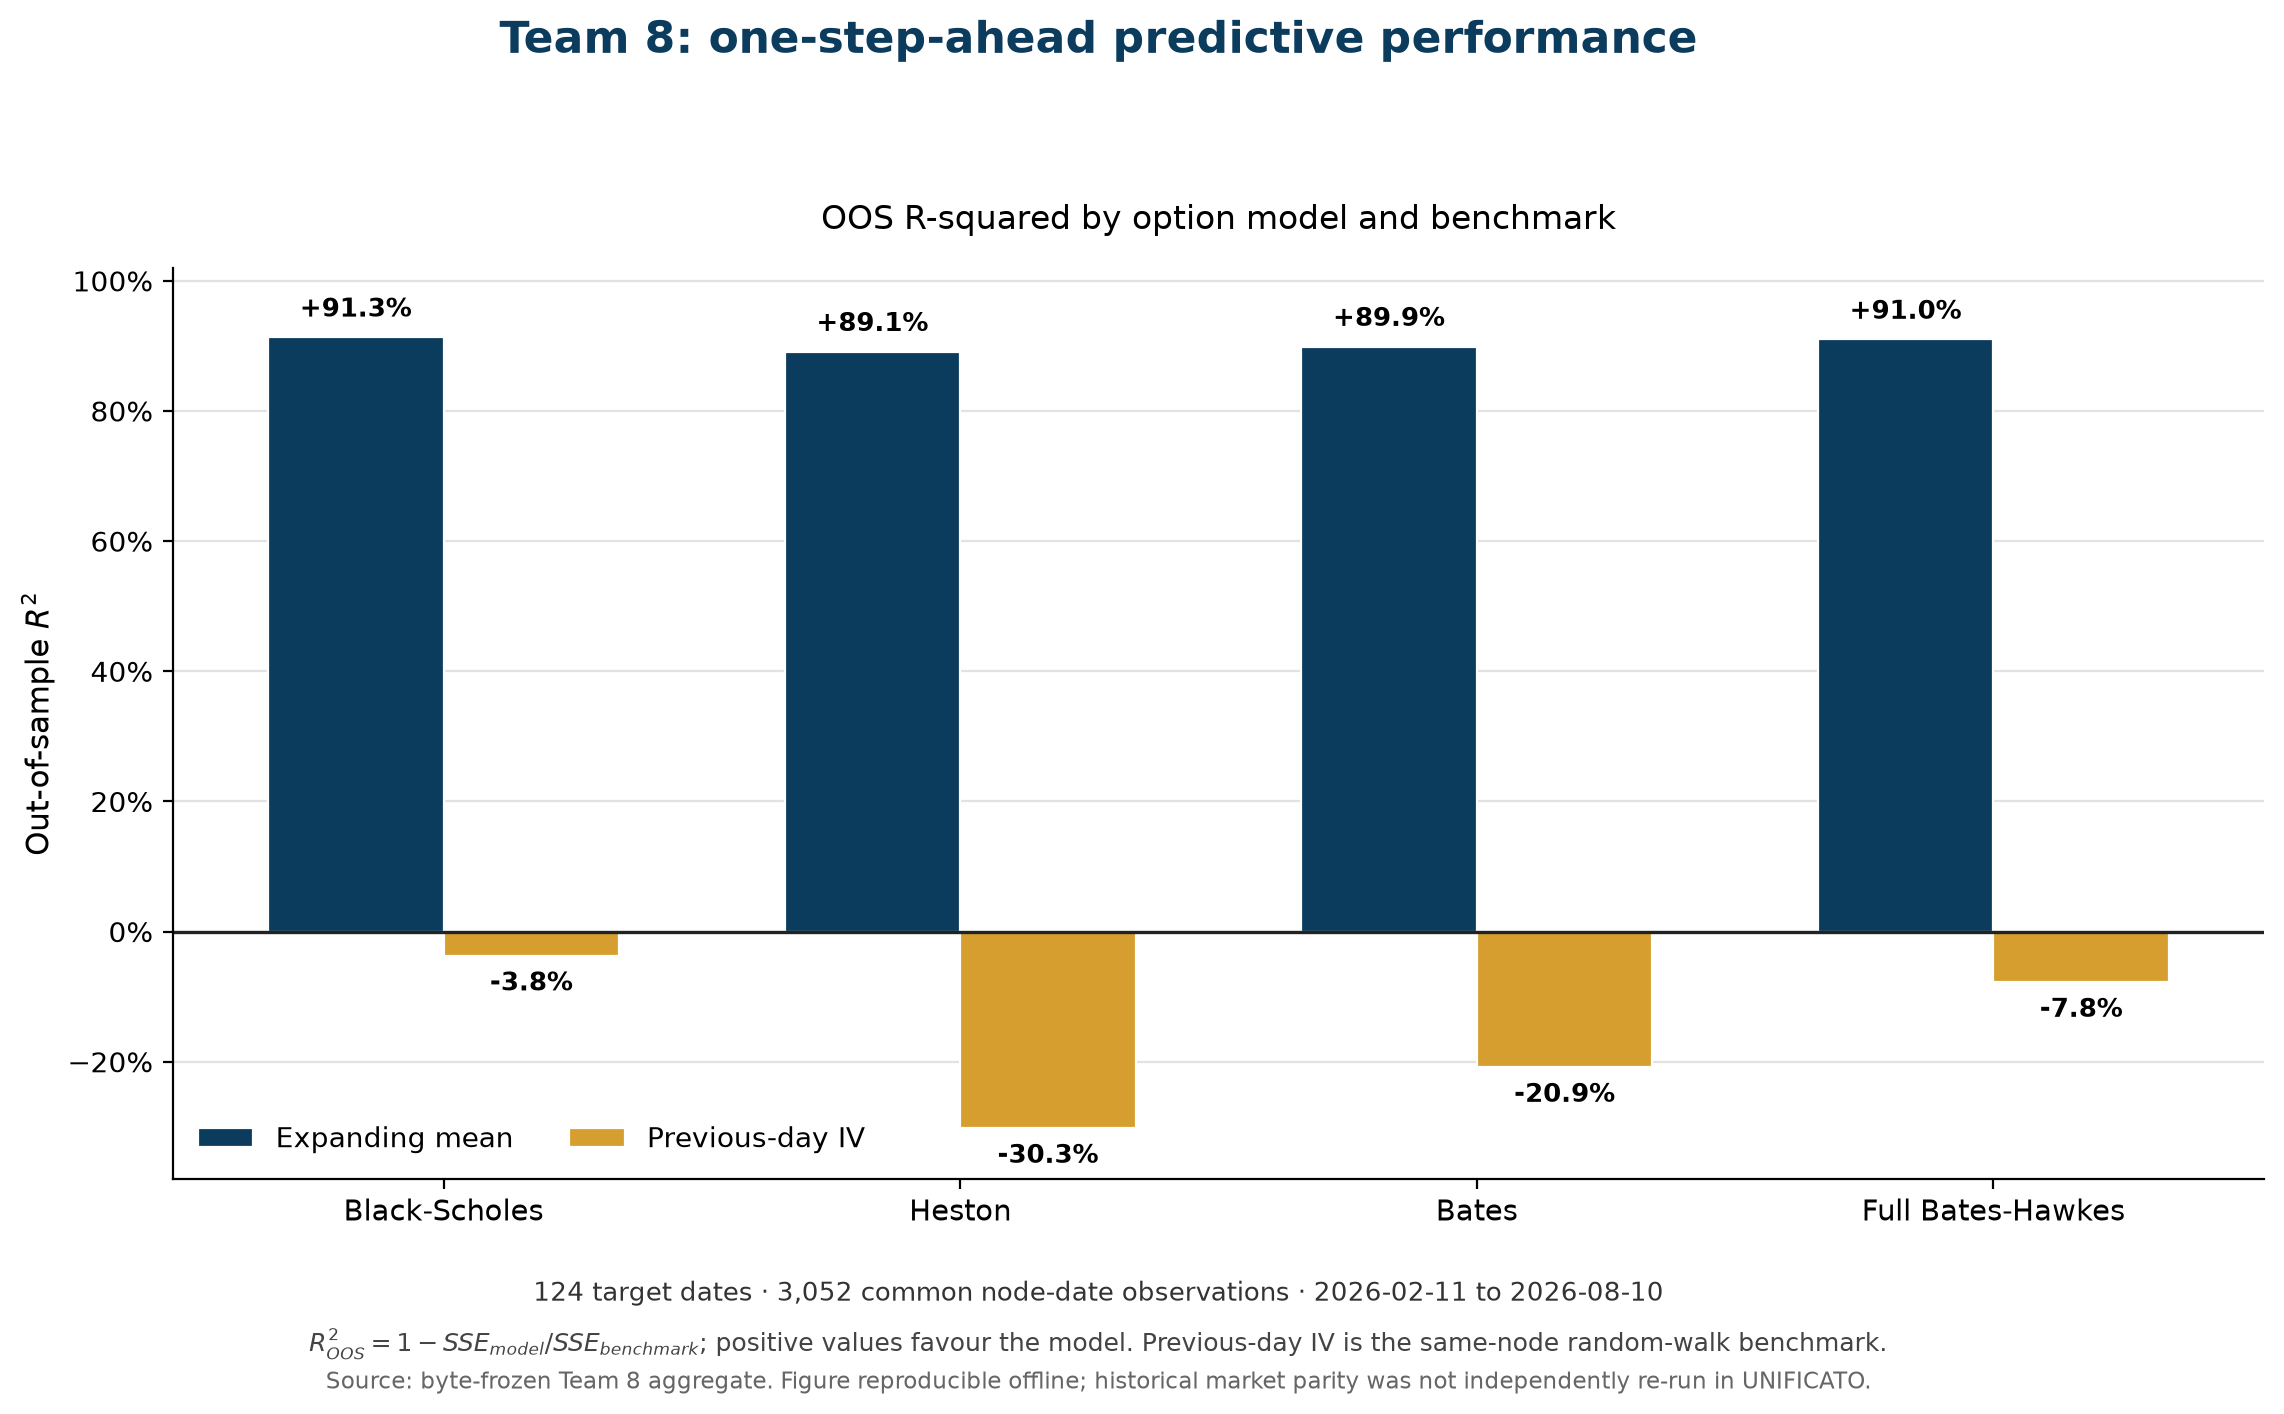
\includegraphics[width=0.98\textwidth]{img/diagnostics/online_oos_r2_by_benchmark.png}
    \caption{Team 8 rolling one-step-ahead out-of-sample \(R^2\) by model and
    benchmark. All four specifications improve on the node-specific expanding
    mean, but none improves on carrying forward the previous day's normalized
    IV surface. The chart is rebuilt offline from the byte-frozen aggregate;
    it does not claim independent historical market-parity replication.}
    \label{fig:online-oos-r2}
\end{figure}
}{%
\gapbox{The Team 8 OOS \(R^2\) chart is withheld unless it is regenerated from
the frozen online-validation metrics and passes the sample and identity checks.}%
}

All four models beat the expanding mean, and the HAC differences are significant. The stronger random-walk benchmark reverses the conclusion: no model has positive \(R^2_{OOS}\) against yesterday's surface. Black--Scholes has the lowest pooled RMSE, while full Bates--Hawkes is close; their pairwise \(R^2\) favors Black--Scholes by 3.77\%, but the HAC difference is not significant (\(p=0.421\)). Full Bates--Hawkes beats Heston by 17.23\% pairwise and the difference is systematic (\(p=1.06\times10^{-4}\)); its 10.81\% advantage over Bates is not significant (\(p=0.126\)). Thus added structure helps some comparisons, but daily IV persistence remains the hardest benchmark.

Rolling parameters also expose identification pressure. The full model's branching ratio has a median of 0.0203, close to the imposed 0.02 floor, and some jump-size parameters approach lower bounds. The current cross-section estimates stronger self-excitation, but the online history does not support presenting that current estimate as a stable law.
\subsubsection{Fixed-Cutoff Six-Month Stress Test}

The earlier frozen-parameter design is retained as a deliberately harsher robustness check, not as the primary online test. Parameters are estimated once on 10 February 2026 and never refitted during 27 weekly holdout surfaces through 10 August. Against the prevailing mean, \(R^2_{OOS}\) is 46.48\% for Black--Scholes, 44.60\% for Heston, 45.08\% for Bates, and 52.41\% for full Bates--Hawkes. The full model has the lowest frozen-parameter RMSE and significantly lower weekly loss than Heston and Bates, but not Black--Scholes. This stress result measures six-month parameter stability; it does not replace the current-snapshot calibration used by the controlled Barrick comparison.


% ===============================

The preceding model chapters described calibration, constraints, residuals, and smile slices in one place. This chapter checks whether those calibrated models behave sensibly on the option surface. It therefore collects the residual heatmaps, smile fits, and Bates--Hawkes visual diagnostics after the scalar model comparison has already been reported.
\subsection{What the Diagnostics Say Operationally}

The diagnostic layer should be read as a quality-control stage:

\begin{itemize}[leftmargin=8mm, itemsep=2pt]
    \item \textbf{Surface plots} show the empirical object being fitted.
    \item \textbf{Sampling plots} show which market observations are used for calibration and interpolation tests.
    \item \textbf{Residual heatmaps} show whether errors are random-looking or structurally concentrated.
    \item \textbf{Smile slices} show whether the fitted model has a plausible shape within each maturity bucket.
\end{itemize}

% Team 8 evidence regenerated by the unified branch. The rolling OOS figure is
% rendered from a frozen aggregate CSV because licensed option bars are local-only.

\subsubsection{Regenerated market-input and return evidence}

The scalar calibration errors reported above are interpretable only together
with the empirical objects that generated them. Figure~\ref{fig:t8-market-inputs}
shows the dated Treasury proxy and the structured option sample rebuilt by the
unified branch from the 2 September 2026 Team 8 snapshot. The raw licensed rows
remain local and Git-ignored; the figures and aggregate calibration outputs
carry hashes in the code-run manifest.

\begin{figure}[H]
    \centering
    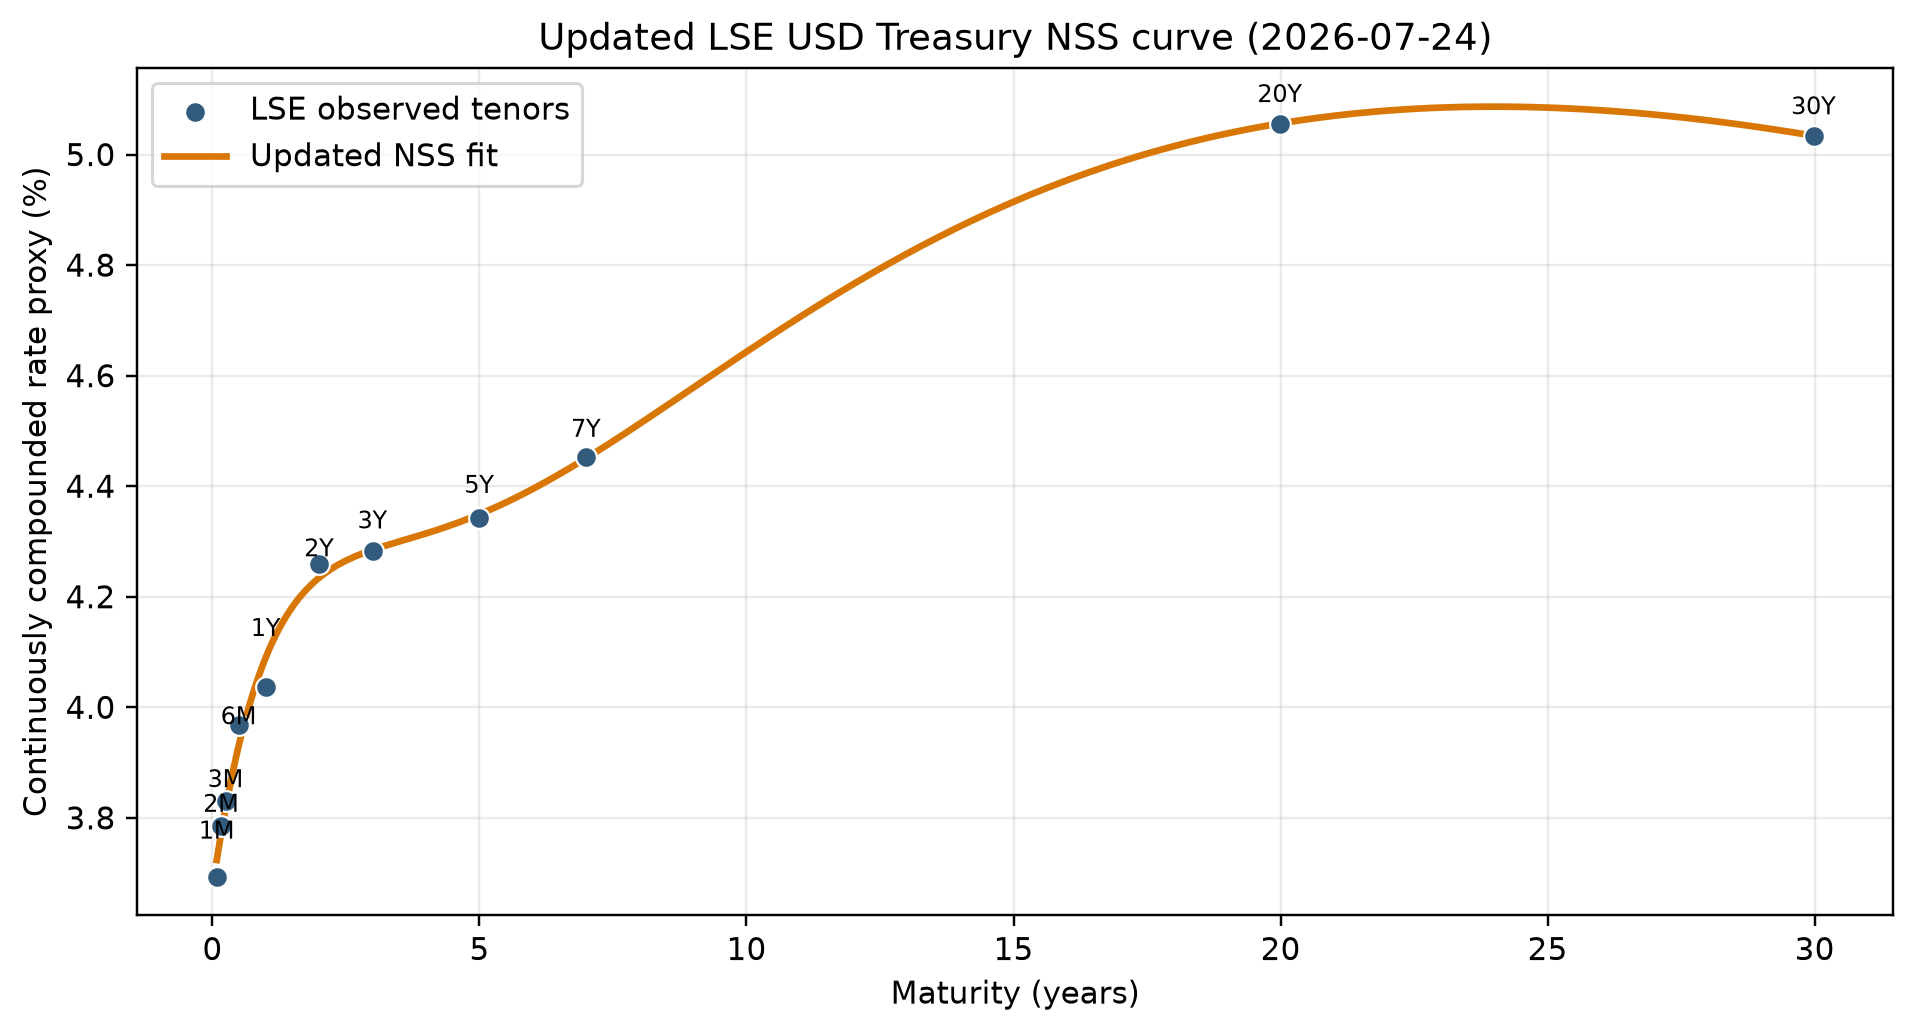
\includegraphics[width=0.82\textwidth]{img/team8_empirical/usd_treasury_curve.png}

    \vspace{4mm}
    
\includegraphics[width=0.88\textwidth]{img/team8_empirical/sampling_comparison.png}
    \caption{Team 8 calibration inputs. Top: 14 same-date continuously compounded U.S. Treasury proxies and their NSS fit
on 2 September 2026. Bottom: the CC64 sample selected from 605 eligible GLD calls
across 12 expiries and 146 strikes; the retained contracts span eight expiries
and 20 strikes. The colours encode observed
    implied volatility; the node layout, rather than an interpolated sheet,
    is the actual object passed to the optimizer.}
    \label{fig:t8-market-inputs}
\end{figure}

The historical GLD return series supplies a different diagnostic from the
option cross-section. It is observed under the historical data-generating
process and is used only to test Gaussian adequacy, not to estimate a physical
drift or to rank option-pricing models. Figure~\ref{fig:t8-return-normality}
shows both the central concentration and the tail departures that motivate a
variance-and-jump model stack.

\begin{figure}[H]
    \centering
    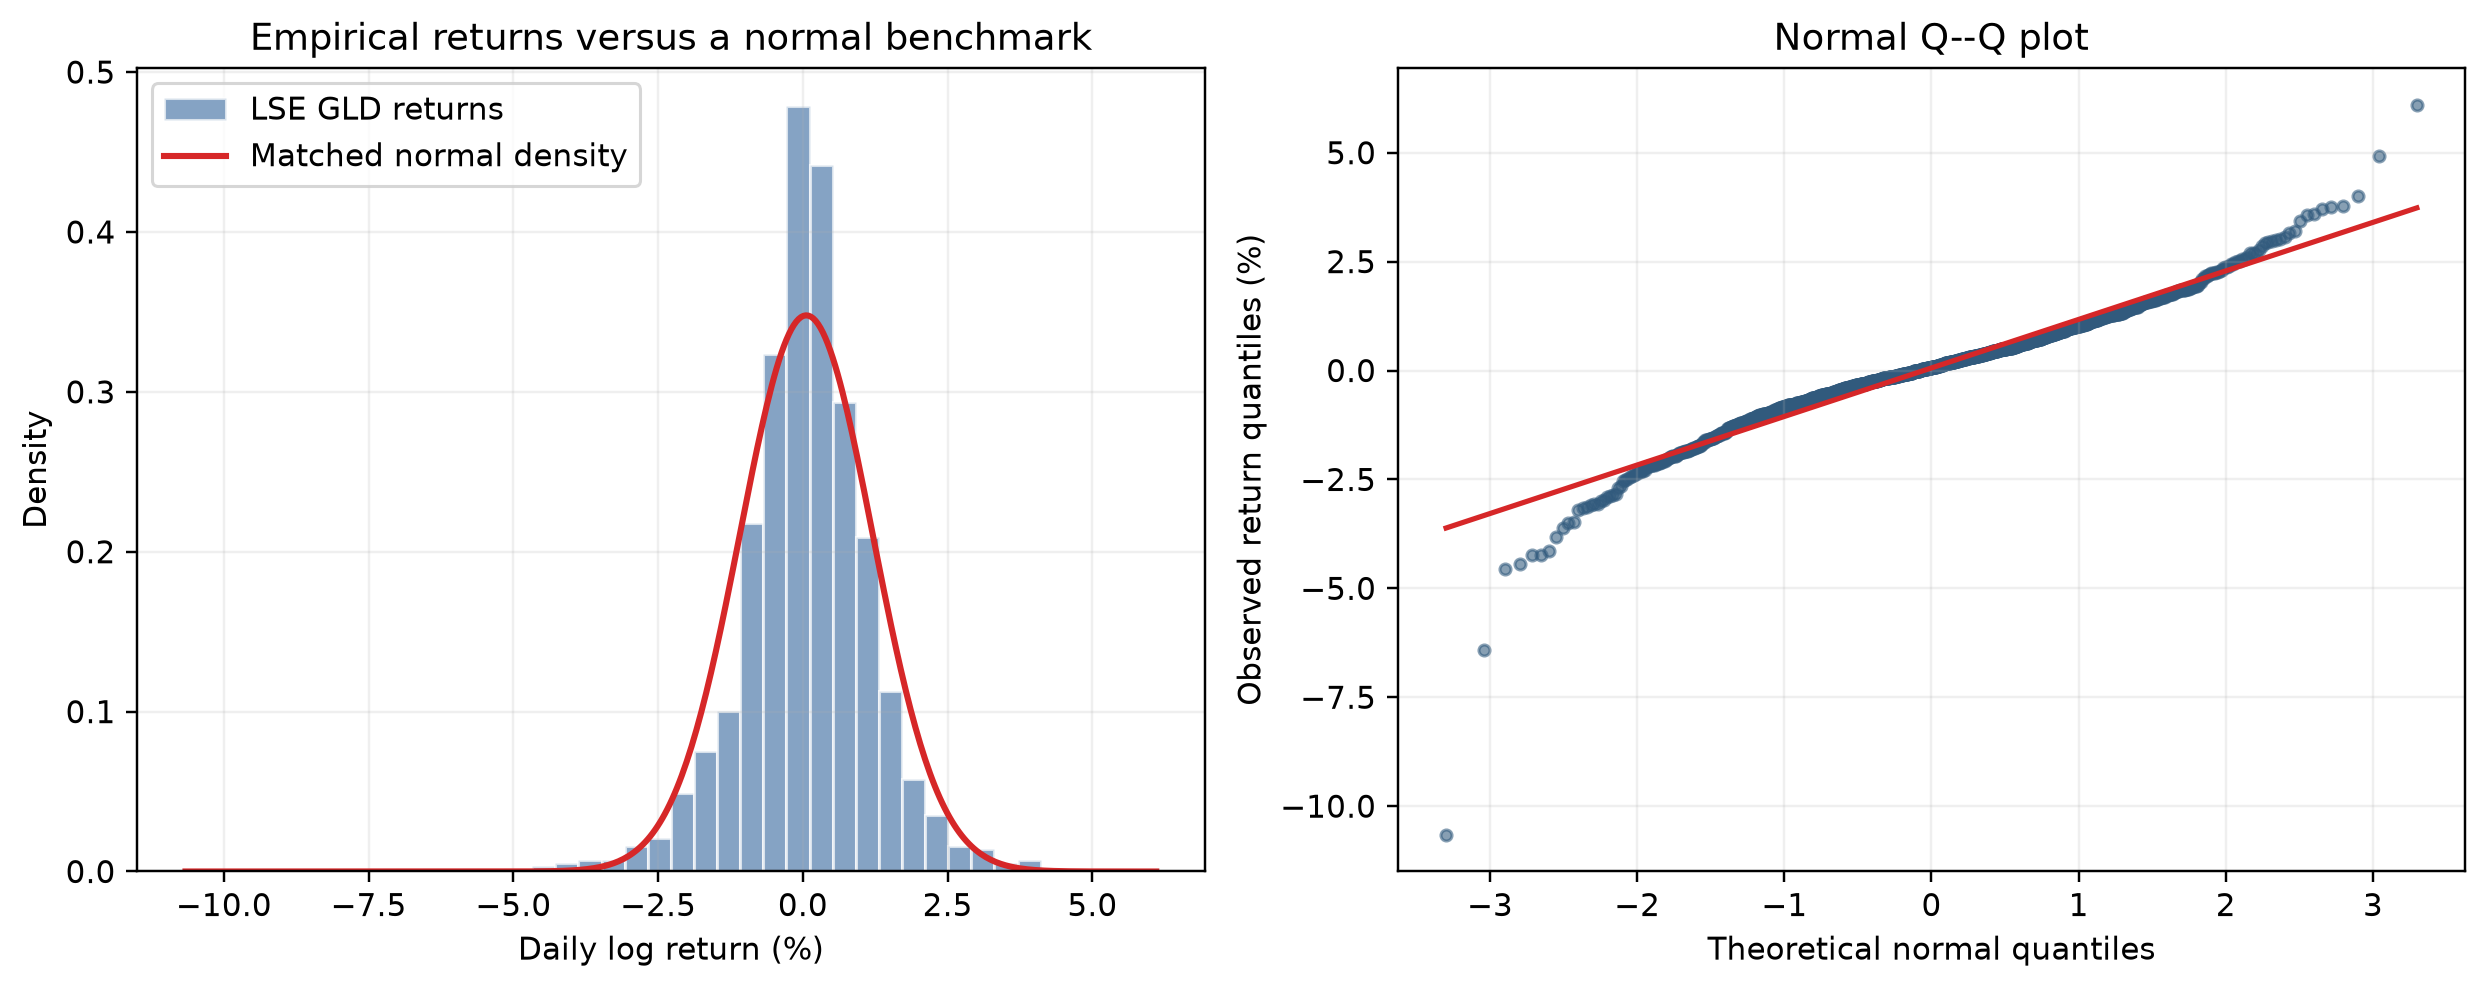
\includegraphics[width=0.96\textwidth]{img/team8_empirical/gld_return_normality.png}
    \caption{LSE GLD daily log returns from 5 January 2021 to 27 August 2026:
    empirical density against a matched normal law and normal Q--Q plot. The
    sample contains 1,424 observations; the visible tail departures are
    consistent with the formal tests in Table~\ref{tab:t8-return-normality}.}
    \label{fig:t8-return-normality}
\end{figure}

\begin{table}[H]
\centering
\footnotesize
\begin{tabular}{@{}lrrl@{}}
\toprule
Test & Statistic & \(p\)-value & Decision at 5\% \\
\midrule
Shapiro--Wilk & 0.9434 & \(6.25\cdot10^{-23}\) & Reject normality \\
Jarque--Bera & 3499.31 & \(<10^{-300}\) & Reject normality \\
D'Agostino \(K^2\) & 322.83 & \(7.90\cdot10^{-71}\) & Reject normality \\
\bottomrule
\end{tabular}
\caption{Normality tests for the 1,424 daily GLD log returns. Sample skewness
is \(-0.733\) and excess kurtosis is \(7.570\). Rejection motivates richer
dynamics but does not by itself select Heston, Bates or Bates--Hawkes.}
\label{tab:t8-return-normality}
\end{table}

\subsubsection{Cross-sectional calibration geometry}

Tables~\ref{tab:t8-model-parameters}--\ref{tab:t8-model-errors} consolidate
the point-in-time fit that is otherwise distributed across the model-specific
sections. All four rows use the same 64 actual nodes, price/IV conversion and
vega-weighted objective; richer models therefore change the state law rather
than the empirical target.

\begin{table}[H]
\centering
\scriptsize
\setlength{\tabcolsep}{2.6pt}
\begin{tabularx}{\textwidth}{@{}>{\RaggedRight\arraybackslash}p{2.35cm}>{\RaggedRight\arraybackslash}X>{\RaggedRight\arraybackslash}p{2.75cm}@{}}
\toprule
Model & Calibrated parameters & Admissibility \\
\midrule
Black--Scholes & \(\sigma=0.25088\). & Positive volatility. \\
Heston & \(v_0=0.06439,\; \kappa=4.05183,\; \theta_v=0.06548,\; \xi=0.72815,\; \rho=-0.01701\). & Feller gap 0.00043. \\
Bates--Poisson & \(v_0=0.06626,\; \kappa=4.05261,\; \theta_v=0.06324,\; \xi=0.67235,\; \rho=-0.03326,\; \lambda=0.24501,\; \mu_J=-0.02767,\; \sigma_J=0.00483\). & Feller gap 0.06053. \\
Full Bates--Hawkes & \(v_0=0.06514,\; \kappa=4.05259,\; \theta_v=0.06346,\; \xi=0.67263,\; \rho=-0.03322,\; \lambda_0=0.03496,\; \bar\lambda=0.56005,\; n=0.55690,\; \beta=2.74823,\; \mu_J=-0.02901,\; \sigma_J=0.02280\). & Feller gap 0.06196; stationary $n<1$. \\
\bottomrule
\end{tabularx}
\caption{Feller-constrained parameters on the current 2 September 2026 Team 8 Chebyshev sample.}
\label{tab:t8-model-parameters}
\end{table}

\begin{table}[H]
\centering
\scriptsize
\setlength{\tabcolsep}{3.1pt}
\begin{tabularx}{\textwidth}{@{}>{\RaggedRight\arraybackslash}p{2.35cm}rrrr>{\RaggedRight\arraybackslash}X@{}}
\toprule
Model & Price MAE & Price RMSE & IV MAE bp & IV RMSE bp & Reading \\
\midrule
Black--Scholes & 0.699 & 0.832 & 73.06 & 97.21 & Common CC64 target. \\
Heston & 0.398 & 0.501 & 38.48 & 49.49 & Lowest current in-sample error. \\
Bates--Poisson & 0.447 & 0.562 & 42.60 & 54.63 & Common CC64 target. \\
Full Bates--Hawkes & 0.410 & 0.514 & 40.76 & 52.97 & Common CC64 target. \\
\bottomrule
\end{tabularx}
\caption{Calibration errors on a common option sample. Heston has the lowest
in-sample IV RMSE; this cross-sectional fit is not an out-of-sample ranking.}
\label{tab:t8-model-errors}
\end{table}

The Full Bates--Hawkes branching ratio is 0.5569, below unity and away from
the former lower bound. This snapshot permits material self-excitation, but
does not establish stable identification across regimes. Heston remains the
current-fit winner; Hawkes is selected separately on rolling OOS performance.

The residual maps in Figures~\ref{fig:t8-residual-atlas-diffusion} and
\ref{fig:t8-residual-atlas-jumps} restore the spatial information hidden by
one RMSE. The continuous colours are interpolation only inside the observed
node domain; the circles identify the observations. Their purpose is to show
where errors remain systematic across maturity and moneyness.

\begin{figure}[p]
    \centering
    
\includegraphics[width=0.49\textwidth]{img/team8_empirical/black_scholes_residual_heatmap.png}\hfill
    
\includegraphics[width=0.49\textwidth]{img/team8_empirical/heston_residual_heatmap.png}
    \caption{Market-minus-model implied-volatility residuals for the two
    diffusion specifications: Black--Scholes (left) and Feller-constrained
    Heston (right). Stochastic variance reduces the scalar loss but does not
    remove structured maturity--moneyness error.}
    \label{fig:t8-residual-atlas-diffusion}
\end{figure}

\begin{figure}[p]
    \centering
    
\includegraphics[width=0.49\textwidth]{img/team8_empirical/bates_residual_heatmap.png}\hfill
    
\includegraphics[width=0.49\textwidth]{img/team8_empirical/bates_hawkes_residual_heatmap.png}
    \caption{Market-minus-model implied-volatility residuals after adding
    discontinuities: Bates--Poisson (left) and Full Bates--Hawkes (right).
    The Hawkes layer lowers the current scalar error, while visible clusters
    remain and residual normality is still rejected.}
    \label{fig:t8-residual-atlas-jumps}
\end{figure}

\begin{figure}[p]
    \centering
    
\includegraphics[width=0.97\textwidth]{img/team8_empirical/bates_hawkes_volatility_smile.png}
    \caption{Observed and Full Bates--Hawkes implied-volatility smiles across
    the eight sampled expiries. The panel view prevents a low aggregate RMSE
    from concealing expiry-specific misses, especially at boundary strikes.}
    \label{fig:t8-bh-smiles}
\end{figure}

The standalone study also compared three Hawkes routes that estimate
different objects. Table~\ref{tab:t8-hawkes-routes} preserves that distinction:
event-time likelihoods are kernel diagnostics, whereas only an option-price
calibration can enter the like-for-like surface comparison.

\begin{table}[H]
\centering
\scriptsize
\setlength{\tabcolsep}{3pt}
\begin{tabularx}{\textwidth}{@{}p{2.25cm}p{2.55cm}p{3.45cm}X@{}}
\toprule
Route & Target & Frozen result & Role \\
\midrule
Exact constant-volatility Hawkes & GLD option surface & \(\sigma=0.22448\),
\(n=0.00460\), objective \(8.674\cdot10^{-5}\). & Transform benchmark;
excludes the Heston variance state. \\
Exponential kernel & Event times & \(n=0.3884\), log-likelihood \(-67.75\),
AIC 141.51, BIC 147.36. & Stable Markovian kernel compatible with affine
pricing. \\
Rough power-law kernel & Event times & \(n=0.4119\), log-likelihood \(-68.03\),
AIC 144.05, BIC 151.86. & Long-memory diagnostic; not the option-pricing
model used in the comparison. \\
\bottomrule
\end{tabularx}
\caption{Historical source-study Hawkes routes; these frozen estimates are not the current September parameter set.}
\label{tab:t8-hawkes-routes}
\end{table}

\begin{figure}[p]
    \centering
    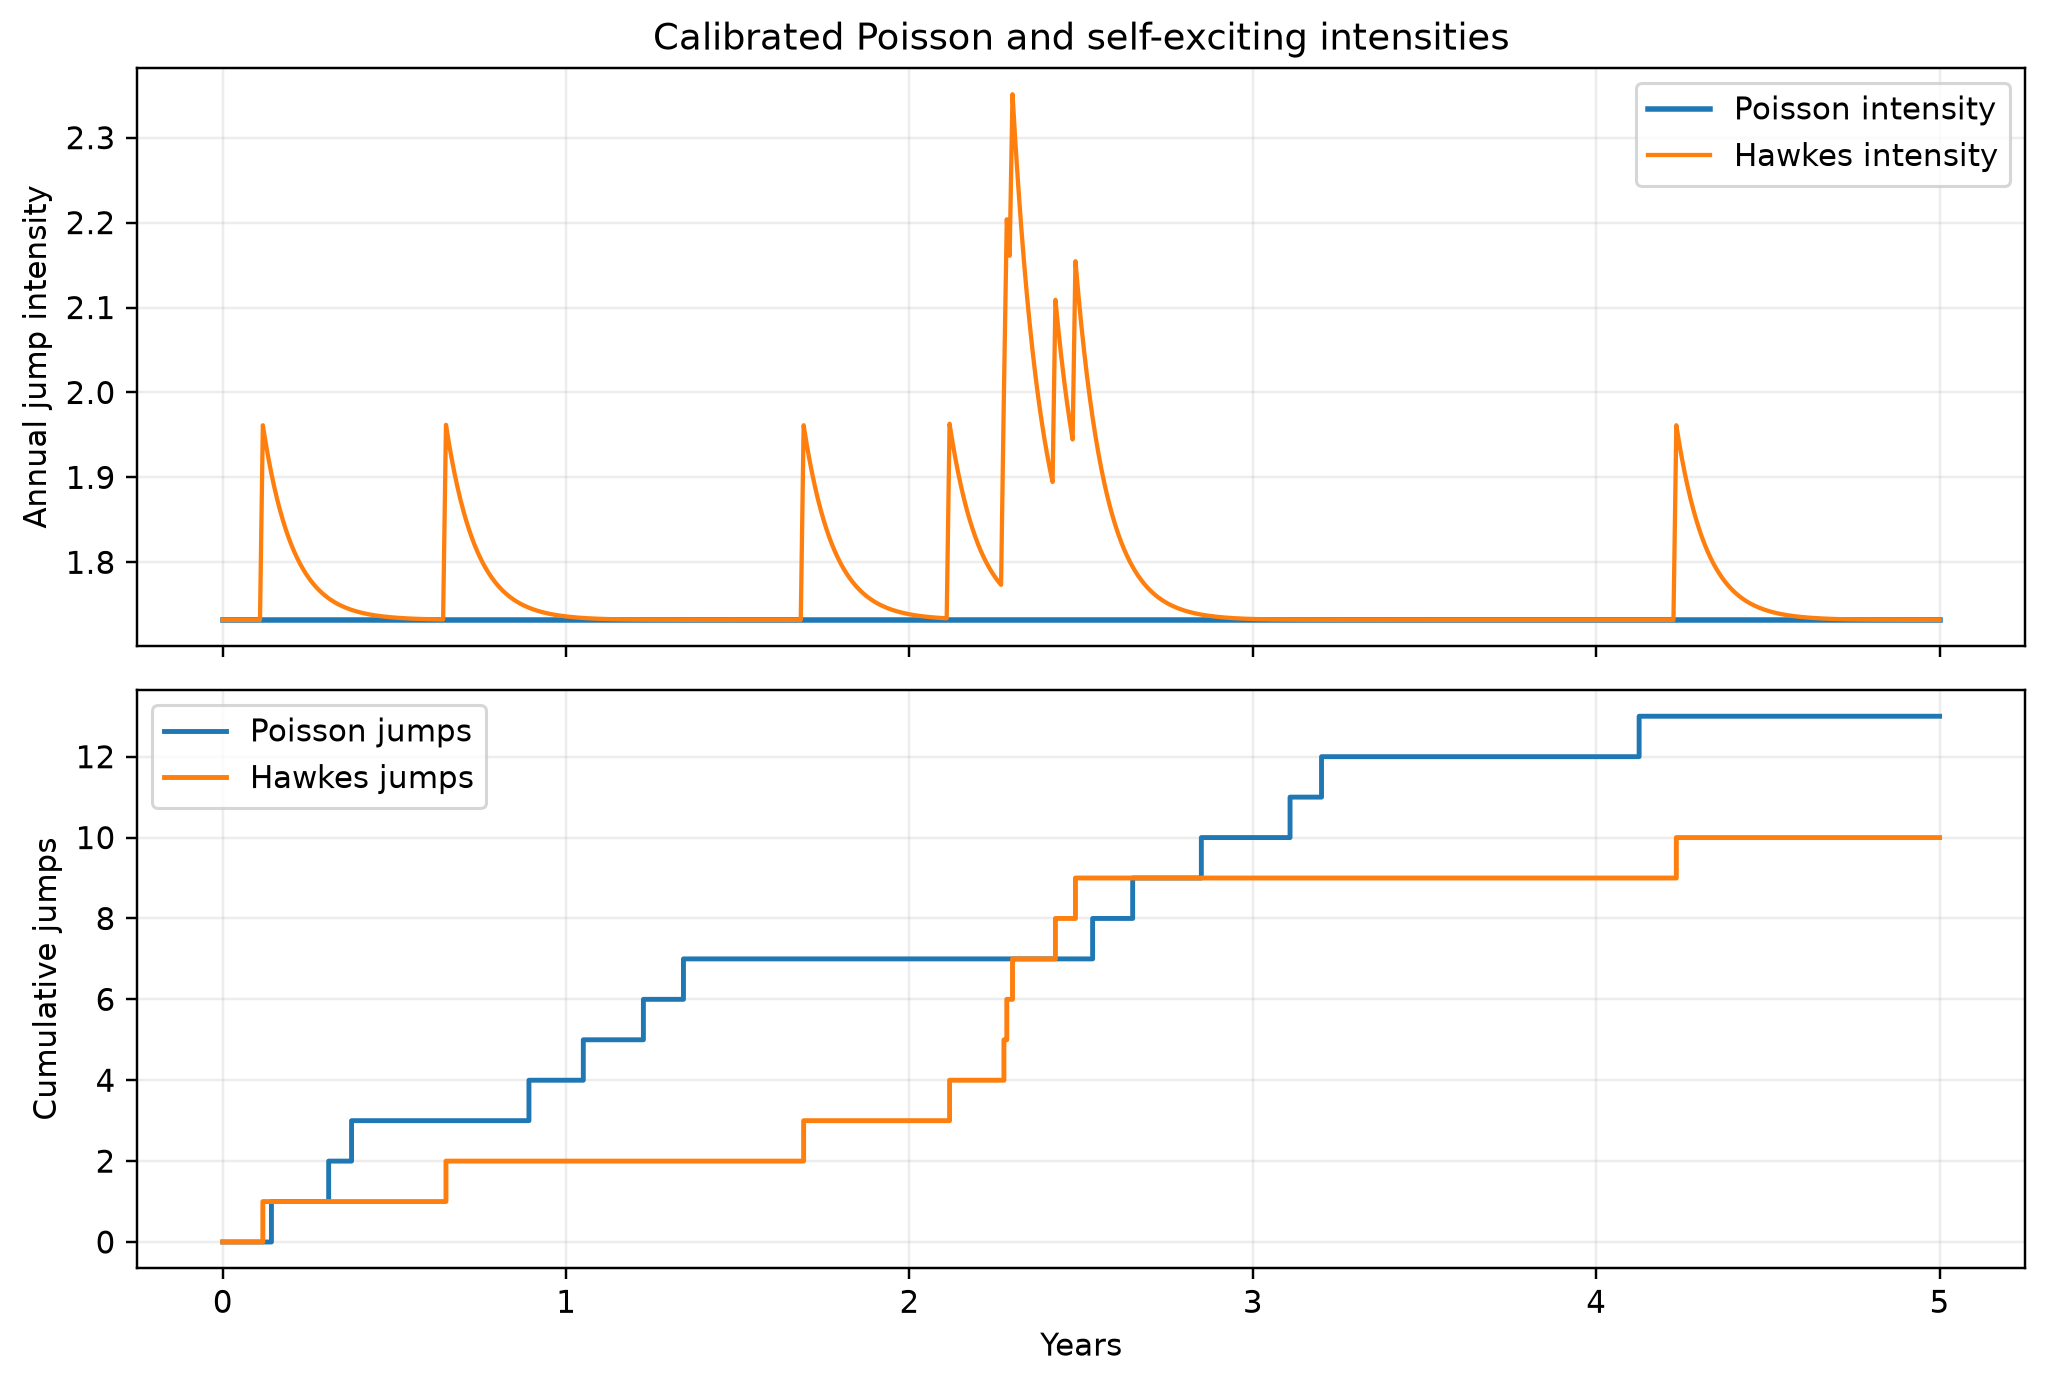
\includegraphics[width=0.94\textwidth]{img/team8_empirical/hawkes_intensity_comparison.png}
    \caption{Constant-intensity Bates jumps versus self-exciting
    Bates--Hawkes jumps regenerated from the current calibration. A Hawkes arrival raises
    near-term intensity, which subsequently decays toward its baseline; the
    lower panel shows the associated clustered event counts.}
    \label{fig:t8-hawkes-intensity}
\end{figure}

\begin{figure}[p]
    \centering
    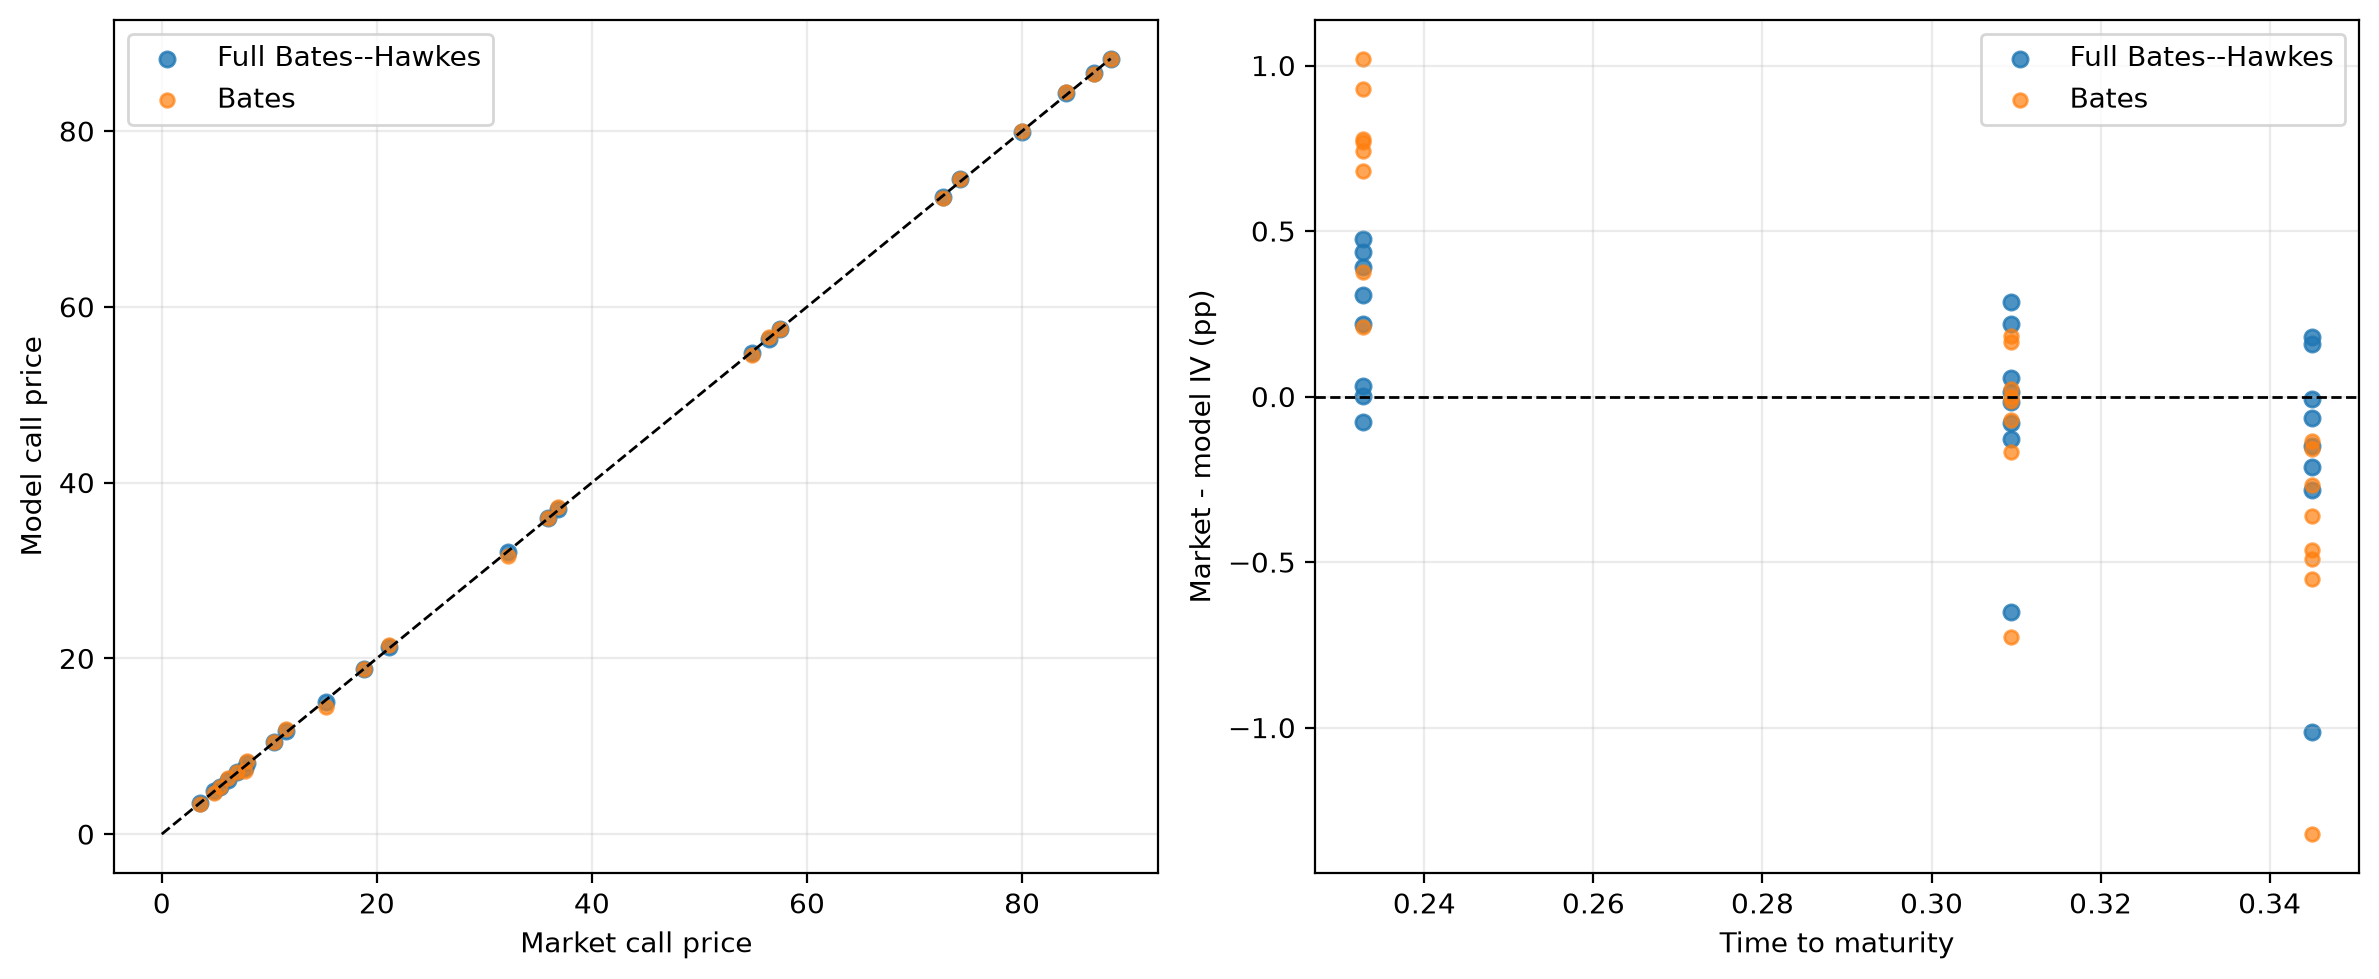
\includegraphics[width=0.98\textwidth]{img/team8_empirical/bates_hawkes_vs_bates.png}
    \caption{Direct current-snapshot comparison between Full Bates--Hawkes and
    Bates--Poisson. The left panel checks option prices against the diagonal;
    the right panel compares market-minus-model IV residuals by maturity. This
    is cross-sectional fit evidence, not proof of predictive dominance.}
    \label{fig:t8-bh-versus-bates}
\end{figure}

\subsubsection{Chronological loss accumulation}

Figure~\ref{fig:t8-welch-goyal} displays the September dense-only rolling
loss differences. The benchmark is the origin cross-sectional mean IV or the
interpolated origin IV surface. Black--Scholes does not beat the mean benchmark;
the three richer models do, but none beats persistence. Full Bates--Hawkes has
the lowest date-equal IV RMSE among the four candidates. These benchmark
comparisons do not establish physical gold forecasting accuracy.

\begin{figure}[p]
    \centering
    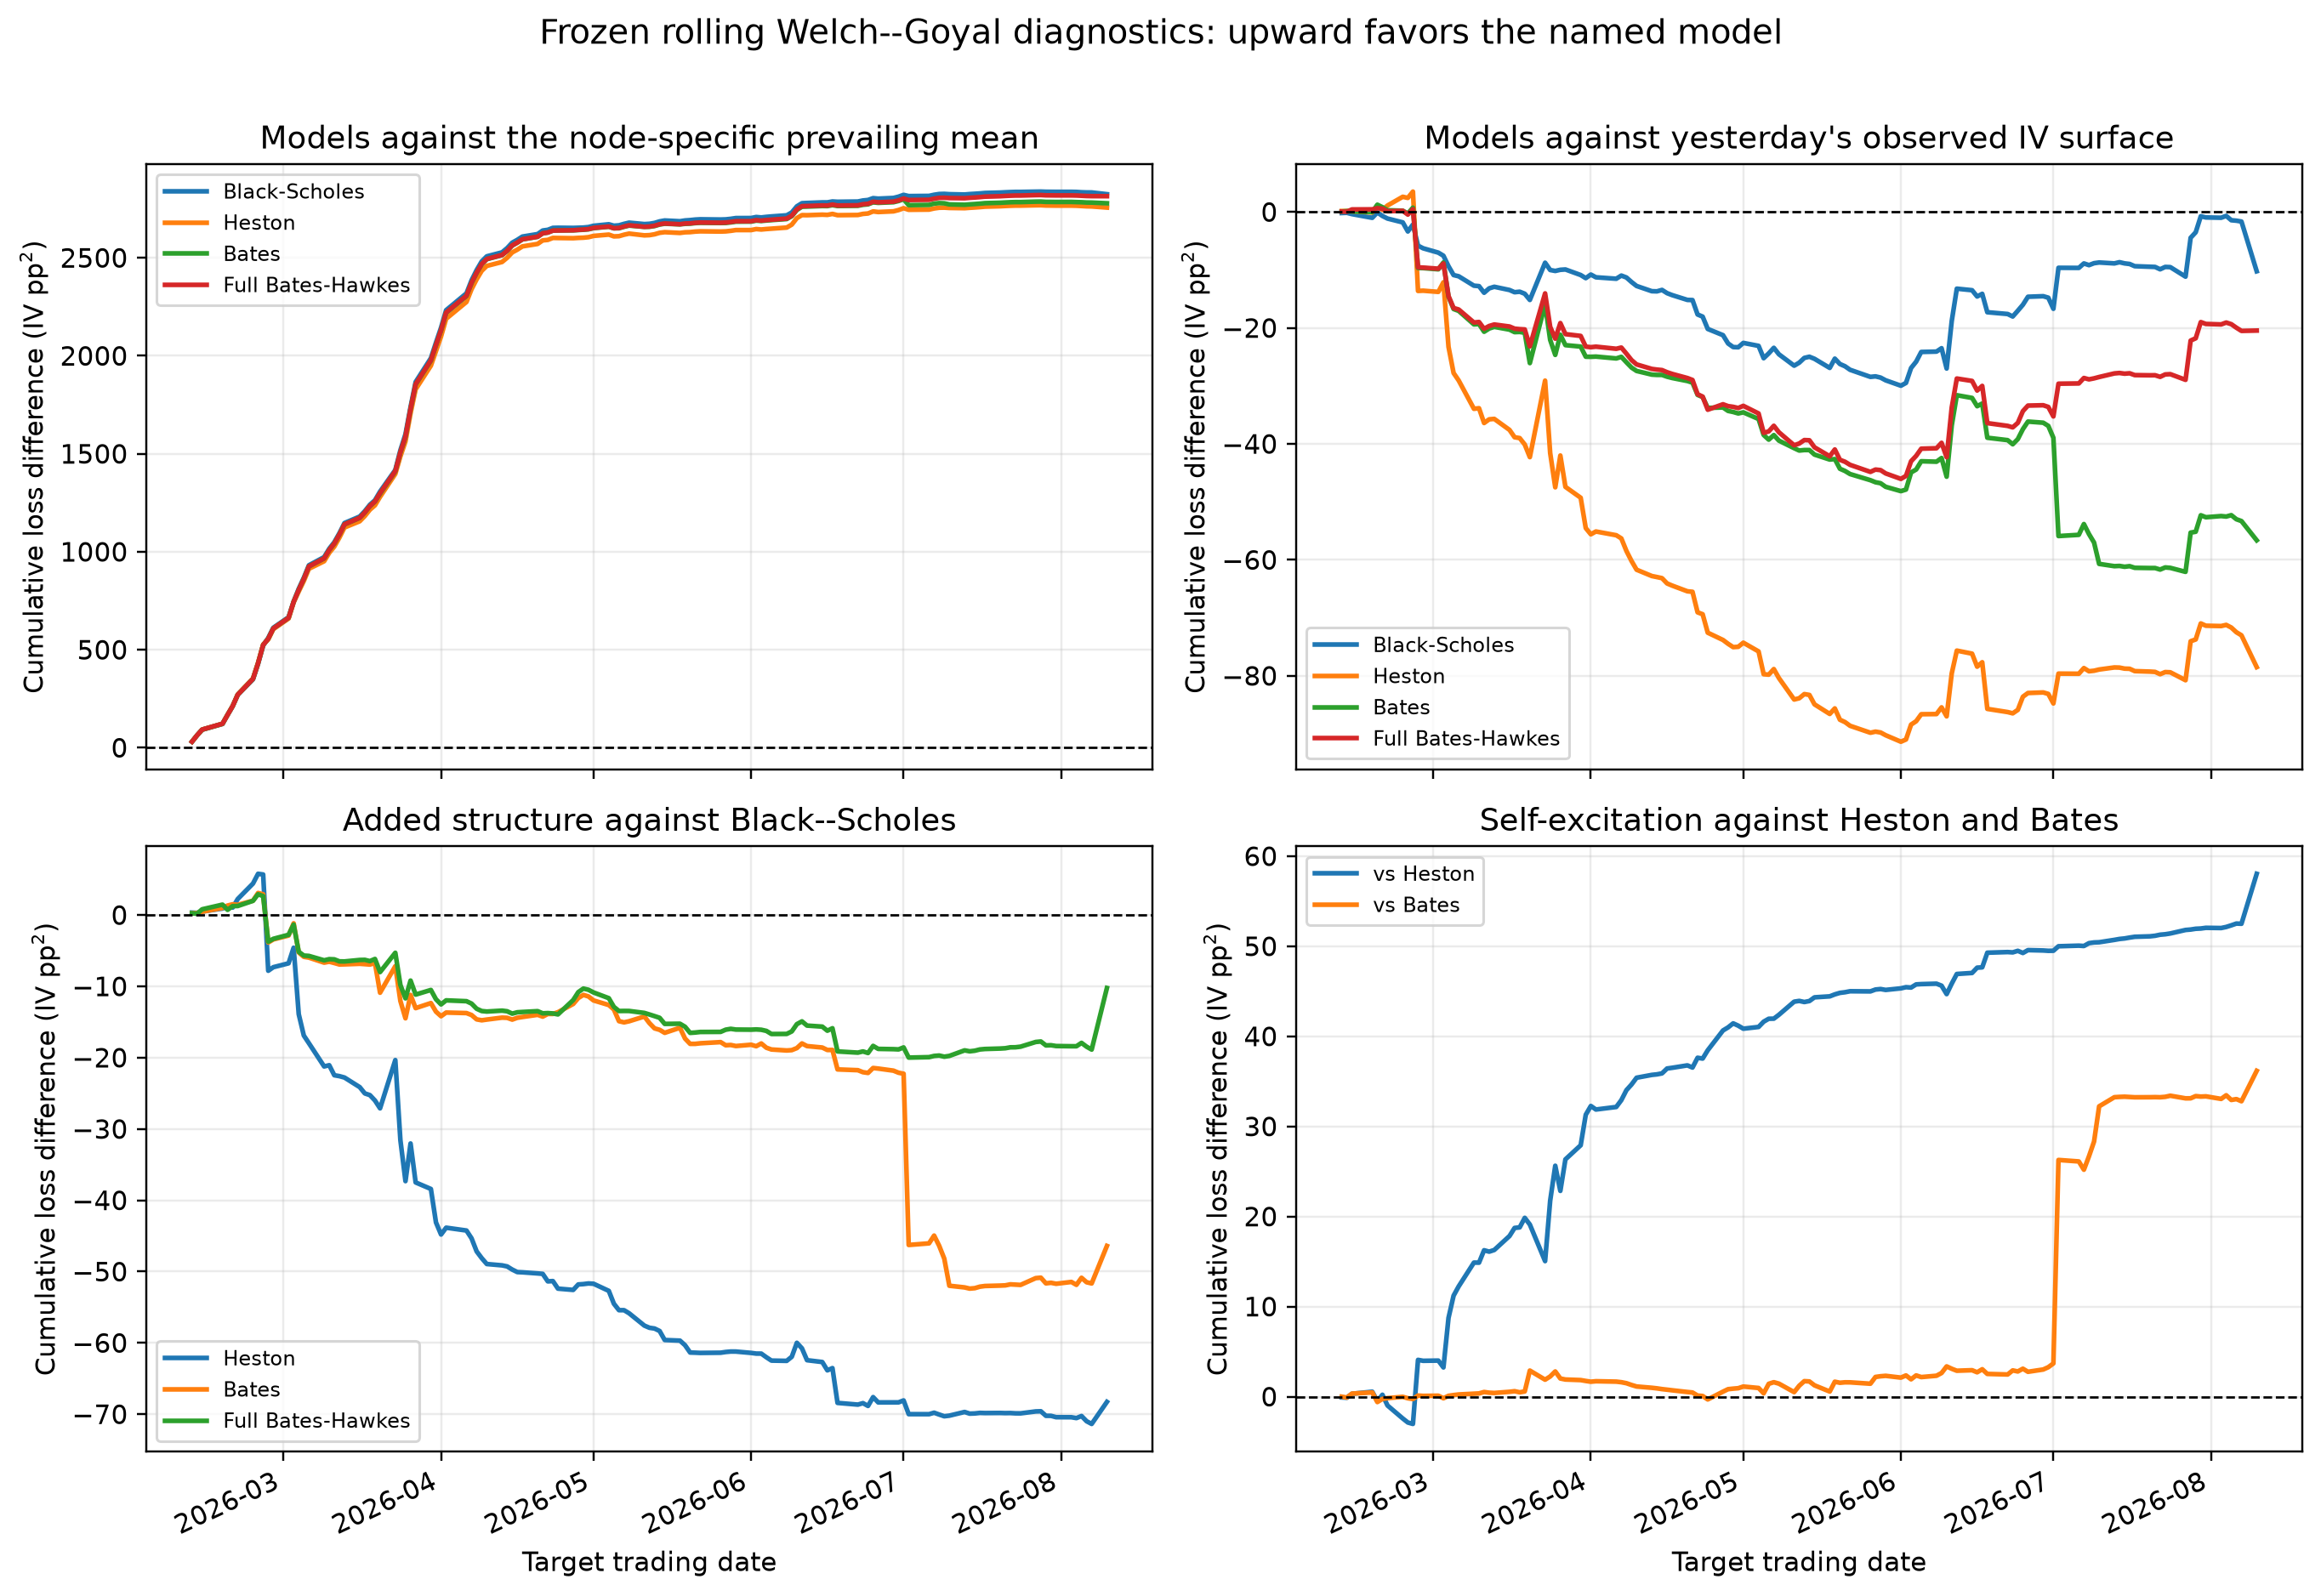
\includegraphics[width=0.98\textwidth]{img/team8_empirical/online_welch_goyal_cumulative.png}
    \caption{Dense-only rolling one-step-ahead Welch--Goyal cumulative squared-error
    differences over the Team 8 validation window, freshly rendered from
    aggregate outputs. Upward movement favours
    the named model relative to the comparator in each panel. The time path
    explains why a positive comparison with the origin mean coexists with
    failure against yesterday's observed IV surface.}
    \label{fig:t8-welch-goyal}
\end{figure}


This is why the article emphasizes diagnostics rather than only model formulas. In applied quantitative finance, a calibrated parameter vector is not self-validating. The model must be checked against the geometry of the observed surface, the admissibility of the parameters, and the stability of the numerical routine. These checks prepare the final step: translating calibrated parameters into simulated gold-price paths.

% ===============================
\subsection{From Calibrated Options to Gold-Price Paths}

Previous work in this track shows why Monte Carlo is the natural numerical language for path-dependent risk and valuation problems, following the same simulation logic developed in standard references such as Glasserman \sourcecitation{Glasserman2003,BarrickArticle3}. Once a stochastic law is specified, many scenarios can be generated and the resulting distribution can be summarized through percentiles, confidence intervals, VaR, CVaR, or other functionals. Earlier company-level modelling also shows why a Barrick framework needs gold-price scenarios. This Team 8 module stops at construction and testing of the price process; Chapter~12 performs the separate corporate integration \sourcecitation{BarrickArticle4,BarrickArticle5}.

The present chapter supplies the price-model block only. In the earlier scenario exercise, a GBM was driven by a Black--Scholes-implied volatility term structure \sourcecitation{BarrickArticle4}. That choice was coherent as a first benchmark, but it inherits the limitations of Black--Scholes: lognormal continuous paths, no stochastic volatility, no jump risk, and no endogenous volatility smile. Heston and Bates provide two natural upgrades because they can be calibrated to the option surface rather than only to a per-maturity scalar volatility.

The simulation layer can reuse the numerical improvements developed in previous Monte Carlo work \sourcecitation{BarrickArticle3}, but it should not repeat that article's comparison between pseudo-random Monte Carlo, quasi Monte Carlo, antithetic variates, and moment matching. Here those tools are inputs. The applied question is different: once a calibrated gold-price law has been chosen, which simulation map is coherent with its state variables?

The accepted implementation uses one Sobol-based simulation interface with moment matching, aligned base seeds and model-specific transformations, while exposing separate policies for diffusion and event-driven blocks. A GBM path needs one Brownian shock, whereas a Bates--Hawkes path needs diffusive shocks, stochastic variance, jump marks and a self-exciting arrival mechanism. The completed design therefore shares what is comparable without pretending that all four models have the same random structure.

% Asset/code block omitted pending provenance acceptance.
\subsection{Monte Carlo Discretization by Model}

The equations below define the implemented model updates. The sampling policy is passed as a simulation configuration rather than hidden inside the financial model itself.

For the GBM baseline, a discrete gold-price update is
\begin{equation}
    S_{t+\Delta t}
    =
    S_t
    \exp\left[
        \left(r_t-q-\frac{1}{2}\sigma_t^2\right)\Delta t
        + \sigma_t\sqrt{\Delta t}\,Z_t
    \right],
\end{equation}
where \(\sigma_t\) is obtained from the Black--Scholes implied-volatility extraction. This is an efficient first approximation, but it compresses the whole option smile into one volatility input per maturity.

For Heston, the Monte Carlo engine simulates both price and variance. Its full-truncation Euler scheme is
\begin{align}
    v_{t+\Delta t}
    &=
    \max\left(
        v_t + \kappa(\theta_v-\max(v_t,0))\Delta t
        + \xi\sqrt{\max(v_t,0)}\sqrt{\Delta t}\,Z_t^v,
        0
    \right),\\
    S_{t+\Delta t}
    &=
    S_t
    \exp\left[
        \left(r_t-q-\frac{1}{2}\max(v_t,0)\right)\Delta t
        + \sqrt{\max(v_t,0)}\sqrt{\Delta t}\,Z_t^S
    \right],
\end{align}
with \(\operatorname{corr}(Z_t^S,Z_t^v)=\rho\). In this version, volatility is no longer an exogenous deterministic curve: it is a simulated state variable calibrated to option prices.

For Bates, the Heston price update receives an additional jump component:
\begin{equation}
    S_{t+\Delta t}
    =
    S_t
    \exp\left[
        \left(r_t-q-\lambda k-\frac{1}{2}\max(v_t,0)\right)\Delta t
        + \sqrt{\max(v_t,0)}\sqrt{\Delta t}\,Z_t^S
        + \sum_{j=1}^{N_t} J_{t,j}
    \right],
\end{equation}
where \(N_t\sim\operatorname{Poisson}(\lambda\Delta t)\), \(J_{t,j}\sim\mathcal{N}(\mu_J,\sigma_J^2)\), and \(k=\exp(\mu_J+\frac{1}{2}\sigma_J^2)-1\). This is the simulation counterpart of the Fourier-pricing model calibrated in the preceding sections. The implemented diffusion block uses moment-matched scrambled Sobol normals; jump counts use an inverse Poisson transform and jump marks use a separate normal block.

\paragraph{Bates--Hawkes extension.}
The Bates--Hawkes model keeps the Heston variance update and replaces the constant jump intensity \(\lambda\) by a stochastic self-exciting intensity,
\[
    \lambda_t = \bar{\lambda}+(\lambda_0-\bar{\lambda})e^{-\beta t}+\sum_{t_i<t}\alpha e^{-\beta(t-t_i)},
\]
so that recent jumps increase near-term jump probability while variance remains stochastic. Event times are simulated by Ogata thinning, the integrated intensity supplies the risk-neutral jump compensator over each time step, and the same full-truncation Heston update used by Bates evolves \(v_t\). The resulting process is therefore a genuine Bates--Hawkes path model, not an exact-Hawkes jump layer attached to constant volatility.

Before the path figures, Table~\sourceref{tab:terminal-path-stats} records the terminal distribution diagnostics. The Bates--Hawkes row uses all parameters from the full call-price calibration in Chapter 6: Heston variance, separate initial and baseline intensities, self-excitation, and lognormal jump marks.

% Asset/code block omitted pending provenance acceptance.


\IfFileExists{img/diagnostics/terminal_return_percentiles.png}{%
% Asset/code block omitted pending provenance acceptance.

}{}

\subsection{Path Simulation Diagnostics}

The calibrated parameter sets are translated into simulated five-year gold-price paths. The Black--Scholes/GBM panel uses a constant implied-volatility input. Heston uses stochastic variance, Bates adds discontinuous Poisson jumps, and the full Bates--Hawkes panel combines a Heston variance process with event-driven self-exciting jump arrivals. All figures and terminal statistics in this section were regenerated after the final Feller-constrained calibration.

% Asset/code block omitted pending provenance acceptance.


\IfFileExists{img/valuation/gold_path_bands_four_models.png}{%
\begin{figure}[H]
    \centering
    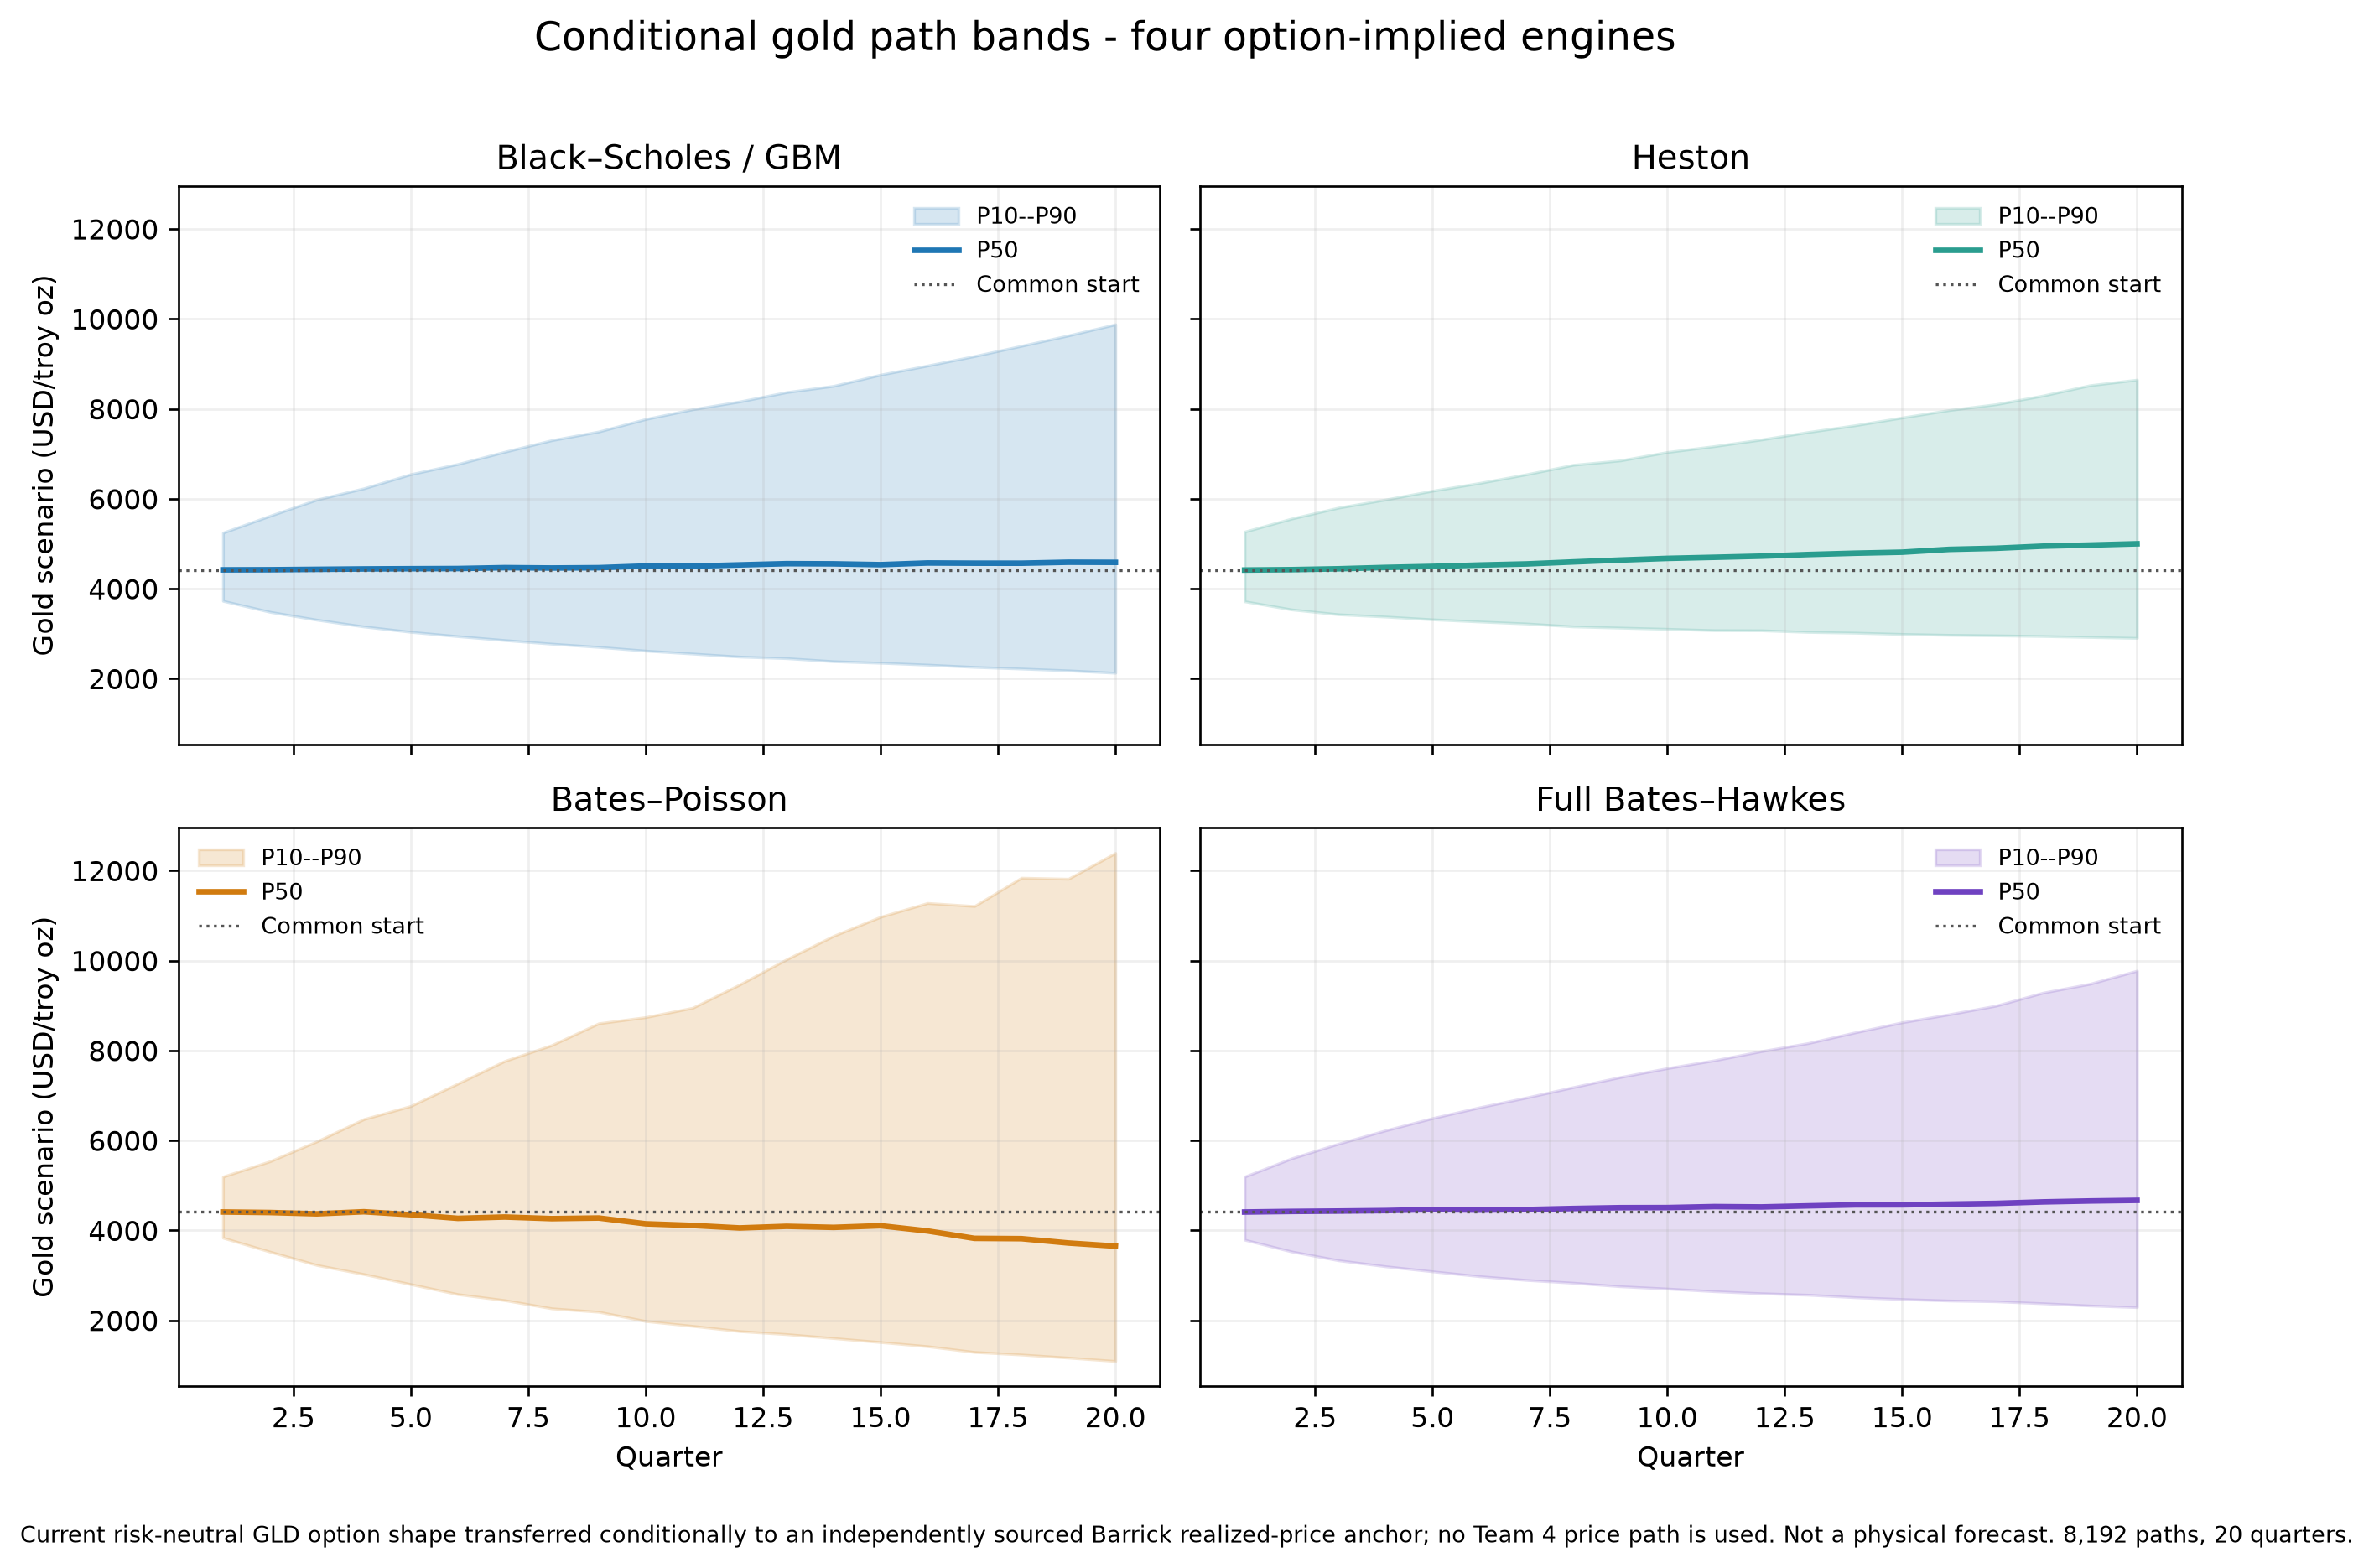
\includegraphics[width=0.98\textwidth]{img/valuation/gold_path_bands_four_models.png}
    \caption{Conditional P10--P50--P90 gold-path bands for Black--Scholes/GBM,
    Heston, Bates--Poisson and Full Bates--Hawkes. The 8,192 paths share the
    common Barrick Q2 2026 realised-price anchor of USD 4,417/troy oz, a
    five-year/20-quarter horizon and aligned base seeds. The option-implied
    shape comes from the current 27 August 2026 Team~8 calibration. Team~4
    price paths are not used. These are risk-neutral conditional scenarios, not a validated
    physical forecast or a Q-to-P mapping.}
    \label{fig:gold-path-bands-four-models}
\end{figure}
}{%
\gapbox{The four-model gold-path bands are withheld unless the accepted
CODE-012 figure bundle and its CSV/JSON sidecars are available.}%
}

The latent states are shown separately so their scales remain readable. Heston, Bates, and full Bates--Hawkes each carry stochastic variance. Bates has a constant annual Poisson intensity, whereas the Hawkes intensity jumps upward after arrivals and decays toward \(\bar{\lambda}\). Keeping volatility, Hawkes jumps, and Bates jumps in three figures avoids compressing a nearly constant intensity beside a much more variable volatility process.

% Selected simulation evidence regenerated by the unified branch.

\subsubsection{Current terminal distribution and latent-state diagnostics}

The current Team~8 diagnostic simulation uses the 2 September calibration,
4,096 paths, 260 steps and the GLD level 402.78 USD/share. Its constant
annual rate is 4.0770\%, as recorded in the diagnostic table. This standalone
state-law illustration differs from the corporate adapter, which restarts at
Barrick's realised-price anchor and uses integral-preserving NSS forward rates
and 8,192 paths. Neither the levels nor the path percentiles are interchangeable.

\begin{table}[H]
\centering
\scriptsize
\setlength{\tabcolsep}{2.45pt}
\begin{tabular}{@{}lrrrrrrrr@{}}
\toprule
Model & Mean & Std & P05 & P50 & P95 & Return skew & Ex. kurt. & Mean jumps \\
\midrule
GBM / BS & 490.549 & 289.852 & 160.071 & 423.839 & 1036.482 & 1.743 & 5.708 & 0.000 \\
Heston & 495.256 & 308.314 & 164.068 & 421.222 & 1087.352 & 2.133 & 9.293 & 0.000 \\
Bates & 496.912 & 310.039 & 161.053 & 421.499 & 1098.107 & 2.069 & 7.779 & 1.259 \\
Full Bates--Hawkes & 494.830 & 300.874 & 164.799 & 425.021 & 1063.213 & 1.901 & 6.477 & 5.206 \\
\bottomrule
\end{tabular}
\caption{Terminal GLD price and simple-return diagnostics regenerated from the
current Team 8 calibration: 4,096 five-year paths, 260 steps and a fixed seed. The jump
models mainly alter tail shape and event counts; these levels are not Barrick
values and are not inputs to the later 8,192-path corporate comparison.}
\label{tab:t8-terminal-path-stats}
\end{table}

\begin{figure}[p]
    \centering
    
\includegraphics[width=0.94\textwidth]{img/team8_empirical/terminal_return_percentiles.png}
    \caption{All integer percentiles 0--100 of five-year simple GLD returns in
    the current Team 8 simulation. The symmetric-log scale retains the
    central distribution while exposing extreme endpoints; the full integer
    percentile tables remain in the source article rather than being repeated
    in the thesis.}
    \label{fig:t8-terminal-return-percentiles}
\end{figure}

\begin{figure}[p]
    \centering
    
\includegraphics[width=0.98\textwidth]{img/team8_empirical/volatility_state_paths.png}
    \caption{Representative annualized stochastic-volatility paths under
    Heston, Bates and Full Bates--Hawkes on a common scale. The plot verifies
    that all three richer engines carry a simulated variance state; the jump
    mechanism does not replace stochastic variance.}
    \label{fig:t8-volatility-state-paths}
\end{figure}

\begin{figure}[p]
    \centering
    
\includegraphics[width=0.68\textwidth]{img/team8_empirical/bates_poisson_jump_paths.png}

    \vspace{3mm}
    
\includegraphics[width=0.68\textwidth]{img/team8_empirical/hawkes_jump_paths.png}
    \caption{Representative jump-state diagnostics. Top: Bates retains a
    constant Poisson intensity while cumulative counts evolve independently.
    Bottom: Full Bates--Hawkes intensity rises after arrivals and decays toward
    its baseline, generating clustered event counts. These path displays
    explain the state difference behind the tail comparison; they are not
    additional forecast observations.}
    \label{fig:t8-jump-state-comparison}
\end{figure}


\IfFileExists{img/diagnostics/volatility_state_paths.png}{%
% Asset/code block omitted pending provenance acceptance.

}{}

\IfFileExists{img/diagnostics/hawkes_jump_paths.png}{%
% Asset/code block omitted pending provenance acceptance.

}{}

\IfFileExists{img/diagnostics/bates_poisson_jump_paths.png}{%
% Asset/code block omitted pending provenance acceptance.

}{}
\subsection{Interface with the Unified Barrick Experiment}

The practical reason for introducing Heston, Bates, and the Bates--Hawkes extension is to provide a stronger gold-price input. This Team 8 module does not estimate Barrick revenues, EBITDA, cash flows or equity value by itself. Its output is narrower: calibrated parameters, option-surface diagnostics and simulated gold-price paths. Chapter~12 connects that output to the separate Team 4 operating layer and Team 5 corporate valuation contract.

The unified experiment connects those paths to production, costs and company-level valuation assumptions through a clean interface:
\[
    \left\{
    S_t^{(m)},\,
    v_t^{(m)},\,
    N_t^{(m)},\,
    \lambda_t^{(m)}
    \right\}_{t=0}^{T},
\]
where \(S_t^{(m)}\) is the simulated gold price, \(v_t^{(m)}\) is the variance path when the model has stochastic volatility, \(N_t^{(m)}\) is the jump count, and \(\lambda_t^{(m)}\) is the jump intensity for the Hawkes extension. The superscript \(m\) denotes the Monte Carlo path. Keeping this boundary explicit prevents the article from confusing two different tasks: modelling the gold price and mapping that price into corporate revenues and value.
\subsection{No Investment Recommendation}

The models in this chapter are research tools. They are used to study the shape of option prices, the numerical behaviour of calibration routines, and the possible distribution of model-driven gold-price paths. They do not provide a recommendation to buy, sell, or hold Barrick Gold, GLD, options, or any related financial instrument. A model-implied price, volatility, or path distribution is conditional on assumptions, data filters, and calibration choices; it is not a trading instruction.

With the simulation boundary and the non-recommendation scope fixed, the unified valuation chapter can use the calibrated price layer without repeating its fit and predictive tests.
